\documentclass[a4paper,12pt]{article}
\usepackage[utf8]{inputenc}
\usepackage[english]{babel}
%-------------------------------------------------------------------------------
% Header and footer configuration
\usepackage{fancyhdr}
\pagestyle{fancy}
\fancyhf{}
\chead{\small Universidad Torcuato Di Tella}
\cfoot{\small \thepage}

% Bibliography management
% See: https://www.overleaf.com/learn/latex/Bibliography_management_in_LaTeX
\usepackage[
backend=biber,
style=alphabetic,
sorting=ynt
]{biblatex}
\addbibresource{references.bib}

\usepackage{graphicx}

\usepackage{hyperref}
\hypersetup{
    colorlinks=false,
    linkcolor=black,
    filecolor=black,      
    urlcolor=black,
}

\usepackage{float}

\usepackage{dirtytalk}

\usepackage{amsmath}

\usepackage{multirow}

\usepackage{caption}
\captionsetup[figure]{font=small}
\captionsetup[table]{font=small}

%-------------------------------------------------------------------------------
\begin{document}

% Front page
\begin{titlepage}
   \begin{center}
        \vspace*{1cm}

        \huge
        \textbf{A Quantamental approach to Bitcoin trading:\\Are we swinging for the Fences?}

        \vspace{0.5cm}
        \large
            
        \vspace{2.5cm}
    \end{center}
    
    \textbf{Student:} Agustin Alba Chicar ag.albachicar@gmail.com

    \vspace{0.8cm}
    
    \textbf{Director:} Pablo Roccatagliata proccatagliata@gmail.com
    
    \vspace{5.0cm}
    
    \begin{center}
        A thesis presented for the degree of\\
        Master in Management and Analytics
            
        \vspace{0.8cm}
        
        \large
        Universidad Torcuato Di Tella\\
        Business school\\
        Argentina\\
        May 2021
    \end{center}
\end{titlepage}

\tableofcontents
\newpage

\section{Abstract}
\label{sec:abstract_en}

Financial companies from all around the world have started to focus their investments in quantitative and algorithmic funds. Those methods run in server applications that execute automatic trades. It is important to distinguish high frequency trading from machine learning trading. The latter is used and analyzed in detail in the present work.

This project explains the development of a trading strategy on Bitcoins based on machine learning techniques. A pipeline proposal is shown which is based on Lopez de Prado's book (\cite{lopez_de_prado}). Some modifications are introduced in the book's pipeline to adjust a momentum primary model on Bitcoins, and to incorporate and study features that would let estimate the size of the primary model bets (secondary model to be trained on top of the first model). The range of features to analyze goes from financial metrics derived from Bitcoin prices and volumes, to Bitcoin and blockchain related features and finally social indexes which incorporate interest and animosity towards Bitcoin itself.

The pipeline proposed in \cite{lopez_de_prado} and implemented in this thesis rigorously handles the dataset, the involved models and finally the posterior backtesting strategies. Details about statistical foundation of the involved methods, algorithm complexity and implementation and domain explanations (such as those related to cryptocurrencies) can be found. The pipeline allows to gather enough information to compare and decide whether a propose strategy is good enough to be implemented. We will use this to compare models that introduce microstructure indexes such as SADF (Supremum Augmented Dickey Fuller) in comparison and conjunction with social indexes.



\newpage

\section{Resumen}
\label{sec:abstract_es}

Empresas financieras en el mundo comenzaron hace ya algunos años a focalizar sus esfuerzos e inversiones en fondos basados en métodos cuantitativos implementados con algoritmos y corriendo en servidores que ejecutan compras y ventas automáticamente. Distinguimos el trading de alta frecuencia del trading basado en aprendizaje de máquina, el cual será objeto de estudio en este trabajo.

En particular, el presente trabajo muestra el desarrollo de una estrategia de compraventa de Bitcoins basada en técnicas de aprendizaje automático. Se propone una implementación del proceso presentado en el libro de Lopez de Prado \cite{lopez_de_prado}. Al proceso anterior se lo modifica para poder incorporar un modelo de momentum sobre Bitcoins y se realiza un estudio sobre los features que permitirán mejorar un modelo secundario (a aprender) para dimensionar los tamaños de las posiciones que la estrategia fundamental (de momentum) proponga. Los features a analizar y comparar van desde métricas financieras del activo subyacente, métricas propias de la tecnología de blockchain y Bitcoin como criptoactivo para terminar con métricas sociales que den información sobre interés y animosidad.

El proceso planteado en \cite{lopez_de_prado} e implementado en este trabajo busca hacer un cuidado riguroso del dataset y los modelos empleados así como posterior backtesting de la estrategia. Este informe detalla los detalles de la implementación tanto a nivel estadístico, algorítmico y de dominio (criptoactivos). A partir de los resultados obtenidos en cada etapa del proceso y finalmente en backtesting podremos analizar el proceso de generación de estrategias sino que también comparar algunas para entender el proceso de selección. En particular, es de relevancia en este trabajo utilizar en contraste índices de microestructura como SADF (Supremum Augmented Dickey Fuller) en comparación y conjunto con los índices sociales.   

\newpage

% @{ Introduction
\section{Introduction}
\label{sec:intro}

\subsection{Problem description}
\label{sec:intro_problem_description}

In the last decades, the notorious technology improvements enabled several industries to grow exponentially. Specifically, in the finance industry we can identify a more recent trend that involves considerable investment efforts in the quantitative and algorithmic trading (see \cite{blackrock_investment} to learn more about the BlackRock case). It is interesting for this research to focus initially on two types of solutions from the above group: high frequency trading (see \cite{hft_intro}), known as HFT, and machine learning for trading \cite{machine_learning_in_finance}. The first group exploits the computational power to arbitrate between securities whereas the other exploits the vast amount of available data through data mining techniques and statistical models.

Different technological improvements enabled the spread of these techniques in the financial industry. First, having more and more data to process required more and more storage which started to cost less and less per storage unit, i.e. \$/GB (\cite{mkomo_cost_per_gb_updated} and the updated version \cite{mkomo_cost_per_gb_updated}). Secondly, the widespread use of mobile devices supported by a more and more connected world (\cite{itu_inet_access}) enabled faster data transfers reducing distance, information lead time, or just broadly speaking the connectivity costs. Another vertical that supported this growth was the raise in computational power which followed Moore's Law \cite{moore_law} allowed more and more complex algorithms to be run in acceptable time (with respect to the needs at hand) enabling old theoretical solutions to have a practical one. For example, Roosenblatt's perceptron dates from 1958 \cite{rosenblatt_perceptron} but it was not after some decades that commercial applications of  those neural networks were made available.

Moreover, the digitalization process and internet access growth \cite{owidinternet} allow more people to participate in markets, access information and make new decisions. The behavior of each economic agent, i.e. individual, in the market became of tremendous importance. It is not anymore a handful of people making decisions but entire societies. Behavioral economic analysis is required to better understand market fluctuations and its evolution. For example, herds and bubbles have been registered for centuries \cite{mackay} to nowadays with two of the most recent and bigger bubbles: the Dotcom bubble \cite{dot_com_bubble} and the US financial crisis in 2008 \cite{financial_crisis_2008}.

In parallel, another phenomenon occurred in 2008 when Satoshi Nakamoto released the Bitcoin paper \cite{bitcoin} and then in 2009 when the Bitcoin software release was published \cite{bitcoin_release}. Pushed by Bitcoin, a new technology ecosystem appeared in the last decade backed up by the blockchain technology. As of February 2021, it is said that over 4,000 cryptocurrencies are available but only twenty of them concentrate the 90\% of the market \cite{statista_crypto}. A document of the World Bank \cite{world_bank_bitcoin} showed that Bitcoin transfers were used for gambling and dark web transactions but it gained attraction in 2016 to ease the process international transactions and then to finance private endeavors. Governments started to experiment with blockchain technologies and what started a decade ago as a niche experiment, it reached a market capitalization of \$1,022,439,972,862 in March 9\textsuperscript{th} 2021 \cite{coinmarket_market_cap_bitcoin}.

Bitcoin and other cryptocurrencies are part of a broader collection named cryptoassets \cite{cryptoassets_book}. The term currency is subject to discussion but omitting the subjective appreciations in the academy in favor or against, we should also consider cryptocommodities and cryptotokens. In \cite{cryptoassets_book} there is a good introduction about these terms and thorough examples for each of them based on their used and recent attraction.

One of the main characteristics about Bitcoin is that its total emission and its emission rate has been defined by design. Every four years the incentive to miners is reduced to a half (it started in 50BTC). This event is called halvening and introduces a structural change in the market because incentives suffer dramatic changes (they are cut down to a half). As it will be later explained, these events involve a high volatility in Bitcoin price as well as a change in market's regime. Strategies around this type of asset should either stay away of halvenings or consider them somehow to avoid important losses. In \cite{lopez_de_prado}, structural breaks are considered to inform models with statistical tests about structural breaks in market that would yield to the "best risk / reward ratios".

This research focuses on a building a strategy development pipeline to build, train and evaluate financial trading strategies and will be exercised with Bitcoin. A primary model based on momentum will provide the main trading signals and a secondary machine learning model will provide the bet size. Financial indexes (such as price, volume and volatility), structural break indexes (such as Supremum Augmented Dickey-Fuller), Bitcoin related indexes (such as stock to flow and number of new addresses ) and social animosity indexes (such as fear and greed index) will be evaluated to improve the secondary model performance. Finally, from backtesting procedures metrics will be determined to assess the strategy performance.

This document has the following outline:
\begin{itemize}
    \item Section \ref{sec:intro} presents the problem to solve, provides context about each involved discipline, comments about the state of the art and defines the scope of this research.
    \item Section \ref{sec:materials} presents the used data sources.
    \item Section \ref{sec:methods} analyzes in detail the features and describes the pipeline and successive iterations over it.
    \item Section \ref{sec:results} presents the results obtained. Pure machine learning model results are separated from financial results.
    \item Section \ref{sec:conclusion} discusses the results and wraps the document.
    \item Section \ref{sec:future_work} presents some unresolved questions and potential lines of work to continue with this research effort.
\end{itemize}
\subsection{Domain}
\label{sec:intro_domain}

This section outlines the theoretical background of each related knowledge domain involved in this research. The following list introduces each subsection:

\begin{itemize}
    \item Subsection \ref{sec:intro_fundamental_trading_strategies} describes the primary model which is a momentum strategy and why it was chosen.
    \item Subsection \ref{sec:intro_crypto_currencies} provides background about cryptoassets, cryptocurrencies and in particular Bitcoin and its ecosystem.
    \item Subsection \ref{sec:intro_financial_machine_learning} introduces the methodology Lopez de Prado explains in \cite{lopez_de_prado}, answers why machine learning is applied and introduces the structure break indexes with strong focus on SADF.
\end{itemize}

As detailed in \ref{sec:intro_problem_description}, the research problem involves many knowledge domains and data from different sources. When working in finance, models need to account for the independent variable time as markets \emph{evolve} with it, i.e. they are dynamic. Among all the available strategies to derive the primary model, momentum was chosen.

\subsubsection{Fundamental trading strategies}
\label{sec:intro_fundamental_trading_strategies}

There are many algorithmic fundamental trading strategies. We can use the classification in \cite{oxford_handbook}:

\begin{itemize}
    \item Impact driven: orders placed in a market affect the price of the stocks based on their volume and the liquidity. Strategies like volume-weighted average price (VWAP) or time-weighted average price (TWAP) can be found in this group.
    \item Cost driven: it not only considers implicit costs as the above but also the explicit costs of the market (e.g. commissions and access fees). We can find implementation shortfall in this group.
    \item Newsreader: based on the semi-strong form efficiency, these algorithms exploit news feeds to derive trading signals out of non-structured data.
    \item Market making: this group exploits the spread in the bid-ask prices.
    \item Statistical arbitrage: strategies in this group focus on two main premises: an asset tends to a \emph{medium} value in the long run (one can profit from deviations) or an asset's price is nonstationary, i.e. it fluctuates without a central value (one can profit from the tendency estimation). Mean reversion and momentum strategies belong to this group.
\end{itemize}

Momentum based strategies focus on deriving when a price starts to rise and drop to derive signals and profit by placing long and short positions on the asset. To derive these events, two different speed (fast and slow) moving average signals are used. The specific timestamps at which the fast and slow averaged signals cross determine an event. A fast signal crossing above the slow signal generates a buy event and the opposite generates a sell signal. A simple variation involves using exponential moving averages instead of simple moving averages and it increase complexity to even entire portfolios behind ETFs like MTUM (\cite{mtum_etf}).

In \cite{value_momentum} the authors explored the performance of momentum with market information of more than 200 years and confirm the strategy generally outperforms the market. In \cite{fact_fiction_momentum} the strategy is demystified in favor of a better comprehension of its strong and weak points. Based on the extensive literature around this strategy in particular, implementation simplicity, compatibility with the available data (no book order available, just stamped prices and volumes) this strategy was chosen to work as primary model.

\subsubsection{Cryptocurrencies}
\label{sec:intro_crypto_currencies}

Satoshi Nakamoto published \cite{bitcoin} with the intention to kick start a decentralized peer-to-peer cash system. However, it did not only do that but also gave birth to a new technology hype which is in continuous evolution and now is heading to mature the stack of services on top of the blockchain technology (\cite{deloitte}).

Let me present a few useful definitions:

\begin{itemize}
    \item Bitcoin: is the software that facilitates the transfer and custody of the bitcoin currency.
    \item bitcoin: a cryptocurrency.
    \item Blockchain: is a transaction database, in this case of the Bitcoin software. It keeps track of all debits and credits of bitcoin applying a very clever and sophisticated fashion (see  \cite{blockchain} for a comprehensive description). 
\end{itemize}

Bitcoin's blockchain technology provides several features:

\begin{itemize}
    \item It is publicly distributed. There are no secrete transactions.
    \item Serves as a historical record of \emph{all} transactions.
    \item It is immutable. Transactions will only be appended in the shape of new information blocks, but the \emph{verified} past cannot be changed.
    \item It is secure, i.e. each transaction is cryptographically verified to ensure valid funds. 
\end{itemize}

Transactions are verified via a \emph{Proof-of-Work} (PoW) algorithm which requires nowadays specialized hardware to process the cryptographic algorithm in a timely and competitive manner. Timely and competitive go hand in hand because the first \emph{miner} in claiming the block hash (result of the PoW) obtains a bitcoin reward provided by the Bitcoin software. The block hash is expensive to obtain but easy to verify what makes the acceptance of a new block a fast process for the entire network.

So far, we have introduced some of the technical characteristics of Bitcoin and supporting technologies. It is important to mention what this payment network provides to users. On one hand we have the privacy. Transactions happen from one wallet \cite{wallet} to another (cryptography comes in to properly describe how they work which is out of the scope of this document) and there is no direct nor easy way to know how is the owner of the wallet. Simply, there is information record about the owner of the wallet operation other than the transaction ledger (the blockchain itself). On the other hand, Bitcoin runs on the internet (using TCP \cite{bitcoin_network}) even on countries with network traffic control which sets the basis to trade worldwide without any regulation.

Another important aspect about bitcoin is the issuance model. Miners are paid every time they append a new block and receive a reward in bitcoins. The reward was initially set to 50 bitcoins and Bitcoin would adjust the mining complexity to get a new block every ten minutes on average. On a 210,000 blocks basis, the reward gets reduced to a half although the complexity keeps on adjusting to have the same throughput of one block every ten minutes. The total amount of bitcoins to be issued is 21 million and we can see in figure \ref{fig:issued_bitcoins} the amount of bitcoins issued by April 2020.

\begin{figure}[!htb]
    \centering
    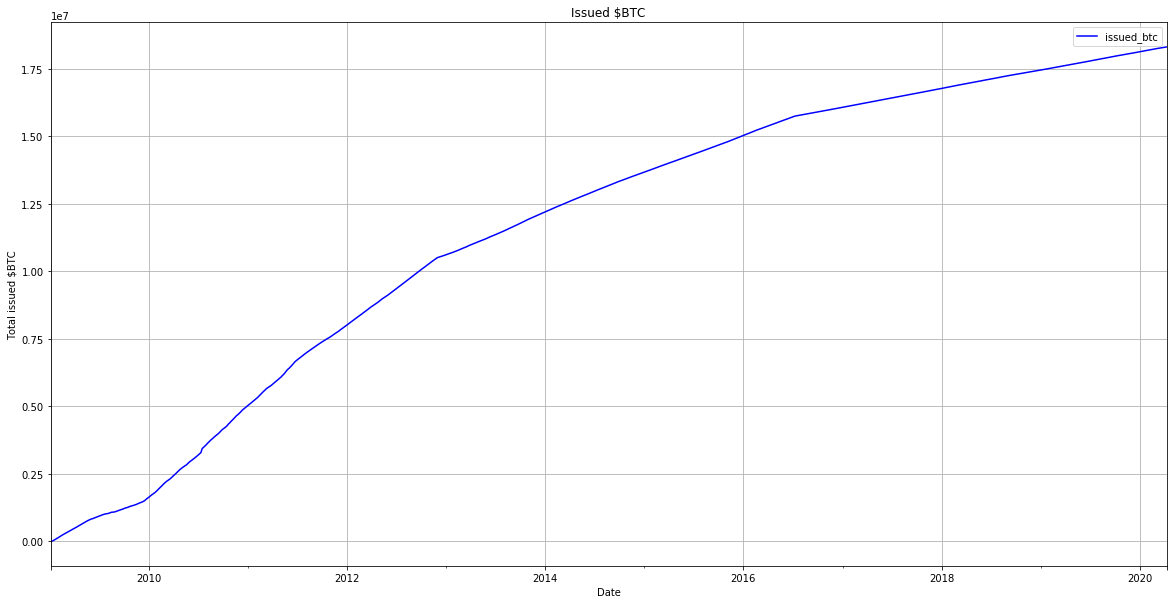
\includegraphics[width=\textwidth]{introduction/images/issued_btc.png}
    \caption{Issued bitcoins through time. Vertical scale is in tenths of millions of bitcoins. Glassnode data.}
    \label{fig:issued_bitcoins}
\end{figure}

And in \ref{fig:issuance} we can see the evolution of bitcoin issuance with time. By April 2021, the total amount of issued bitcoins is 18.66 millions roughly a 88.9\% of the 21 million.

\begin{figure}[!htb]
    \centering
    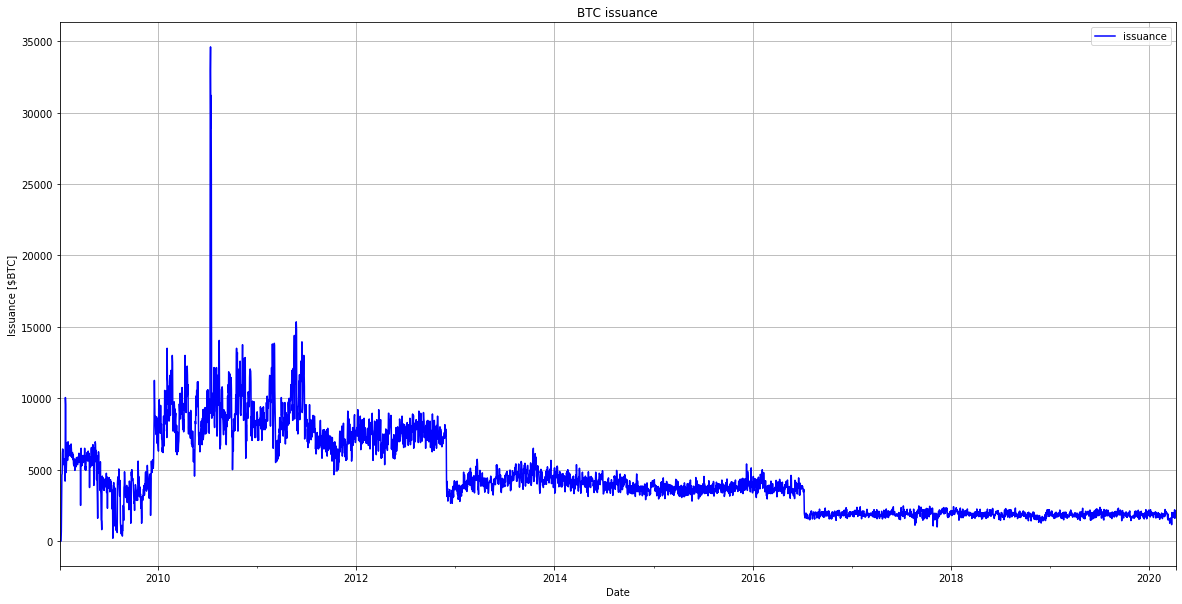
\includegraphics[width=\textwidth]{introduction/images/issuance.png}
    \caption{Bitcoin issuance through time. Glassnode data.}
    \label{fig:issuance}
\end{figure}

As it could be seen in \ref{fig:issuance} and in  \ref{fig:issued_bitcoins} the total number of bitcoins is decelerating. By design, bitcoin is a scarce asset. In \cite{bitcoin_stock_to_flow}, PlanB suggests to use a stock to flow (S/F) model to estimate the value of bitcoin scarcity. In figure \ref{fig:stock_to_flow} the close price series and the S/F ratio are shown to better explain its correlation. In blue we can see the how S/F ratio varies with time and in green we see the close price of bitcoin (note the vertical axis is plotted using a logarithmic scale). In red dotted vertical lines we see the days of the halvings (on 2012/11/28, 2016/07/09, and 2020/05/11). Along this feature (S/F ratio) others will be used that are very specific of the Bitcoin infrastructure and technology. Refer to \ref{sec:material_data_bitcoin_features} for a comprehensive description of the features.

\begin{figure}[!htb]
    \centering
    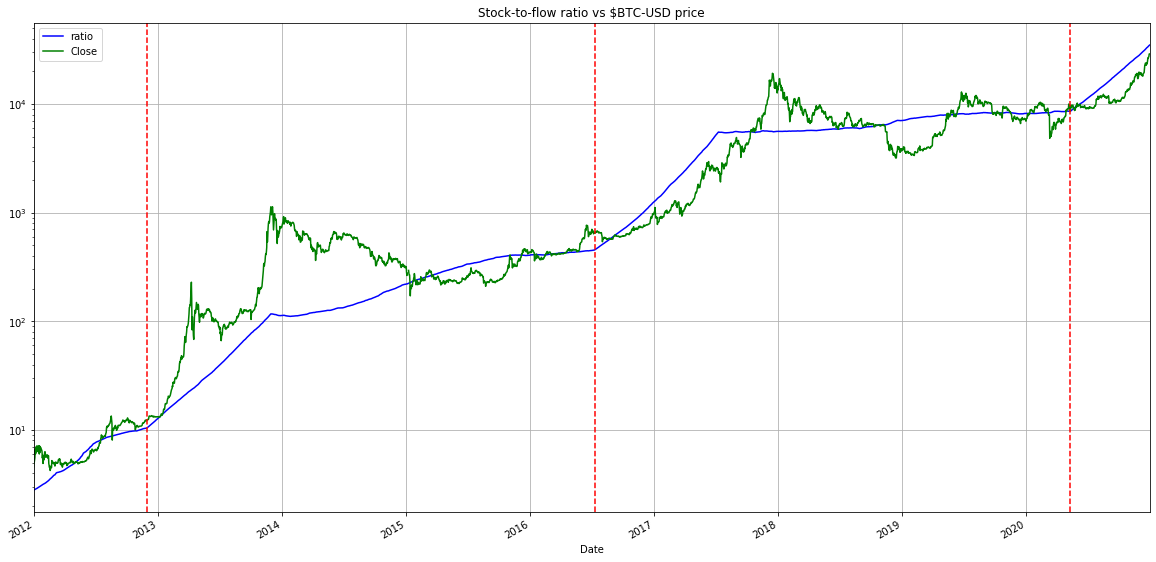
\includegraphics[width=\textwidth]{introduction/images/stock-to-flow.png}
    \caption{S/F ratio versus the close daily price in USD. Plotted in logarithmic vertical scale.}
    \label{fig:stock_to_flow}
\end{figure}

After Bitcoin software was released and gained attraction from different communities, other projects were created \emph{from} it (e.g. the so-called \emph{forks}). Bitcoin is an open source software project (\cite{bitcoin_github}) with a compatible license for both private and public usage which enabled people all around the world to use this technology for multiple purposes such as promotion of new bitcoin-like coins, projects running on top of the blockchain technology, etc.

In this research project we will use bitcoin: the top cryptocurrency by market capitalization as of April 2021 and the first cryptocurrency which started a revolution.

\subsubsection{Financial machine learning}
\label{sec:intro_financial_machine_learning}

This research project involves applied machine learning to finance where it is specifically applied to a trading strategy to learn the size of the position at each bet. In \cite{lopez_de_prado} it is described the procedure to properly develop a machine learning pipeline for a financial application like this one. Lopez de Prado described in \cite{future_of_empirical_finance} problems in financial research publications. The author relates those problems to bad practices and practitioners' ethics sometimes but he also recommended ways to mitigate those issues and their consequences. We could find a similar approach in \cite{lopez_de_prado} with a more in deep explanation of all the aspects which attain the machine learning pipeline to develop.  

As stated before, in this research project we will develop a strategy based on momentum to determine when and how (long vs. short) place our positions. That would define our primary model which follows a secondary model (the machine learning model) to derive the size of the position. Sizing the bet is a two step process: first  we obtain the probability that the buy or sell signal is accurate and second we compute the size of the the bet out of the probability. The model used to derive the probability could be a logistic regression, a tree based model, a neural network, a SVM or whatever model the researcher considers and \emph{finds} that yields better \emph{results}. This research project will focus on comparing some tree based models and evaluating based on \cite{lopez_de_prado} recommendations to mitigate common flaws that will certainly derive into runtime strategy biases and, consequently, losses.

In preparation to train the model, the well known feature engineering stage will be performed. In this case, univariate, bivariate, scaling and other techniques (\cite{feature_engineering}) are relevant but not enough. At least two chapters of \cite{lopez_de_prado} workout in detail two aspect of the time series analysis from a feature point of view: sample uniqueness (explained in section \ref{sec:methods_pipeline_secondary_model}) and sample stationarity (see chapter 15 \cite{time_series_analysis}) vs. loss of memory dilemma (explained in detail in section \ref{sec:methods_features}). One can find thorough explanations of the effects of bootstrap sampling and their effects on the model error (see section 7.11 of \cite{elements_of_statistical_learning}) but it does not usually consider the \emph{duration} of a sample because those in the dataset are often considered both independent and identically distributed (IID) as well as without duration. This is not the case of financial events like this one. Two or more \emph{signals} might overlap due to high volatility in the market or to correlated information. If the model does not take into account that those \emph{signals} refer to the same unique \emph{event} we would incur in unbalanced datasets when training a model due to variations in \emph{event} representativeness. On the other hand, to perform inference we require signals to be stationary but that comes at the expense of removing memory which is essential to obtain the predictive power. Lopez de Prado proposes to use fractional differentiation (see \cite{frac_diff_paper} for the possibly first known occurrence of the method) to determine the minimum differentiation factor $d$ such that the non stationarity null hypothesis of the series is rejected. Hence, some memory will remain in the series and the model can benefit from it.

\begin{figure}[!htb]
    \centering
    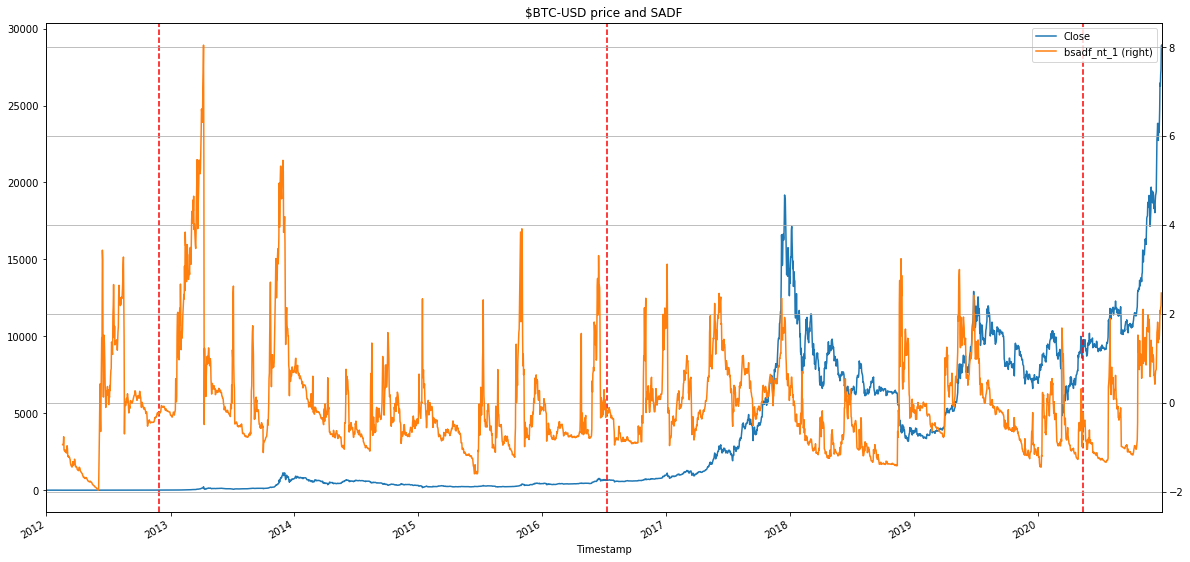
\includegraphics[width=\textwidth]{introduction/images/sadf_vs_price.png}
    \caption{Bitcoin price evolution and SADF index.}
    \label{fig:sadf_vs_price}
\end{figure}

\begin{figure}[!htb]
    \centering
    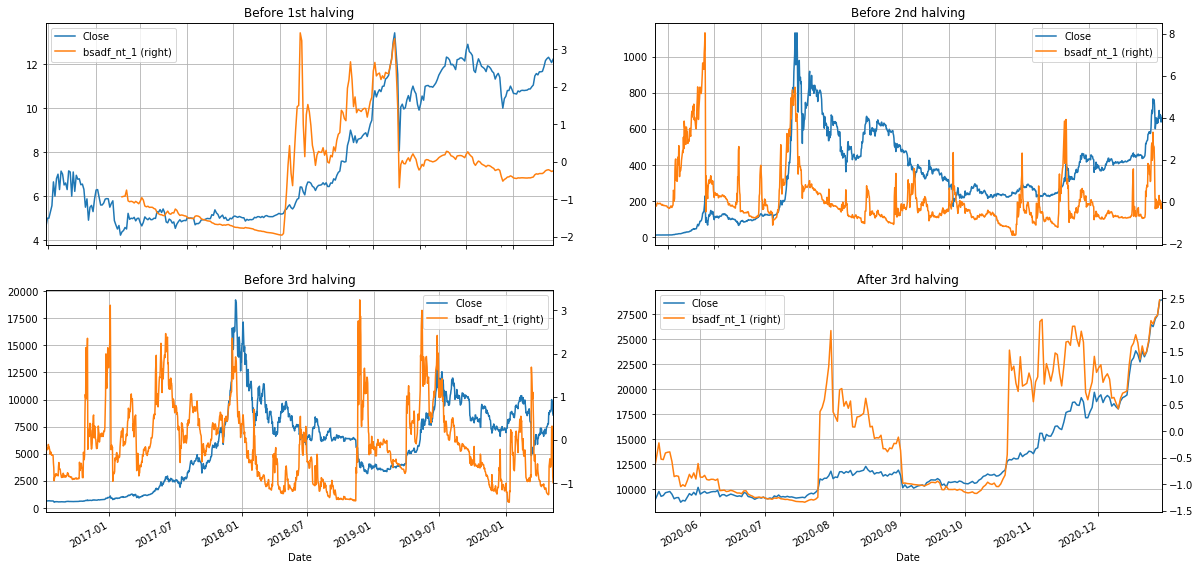
\includegraphics[width=\textwidth]{introduction/images/sadf_per_period.png}
    \caption{Bitcoin price evolution and SADF index by issuance period.}
    \label{fig:sadf_by_halving}
\end{figure}

In \ref{sec:intro_crypto_currencies}, the Stock to Flow model and halvings were introduced. The scarcity model and the issuance scheme imply regime breaks in the price series. Those events are called \emph{structural breaks} and specific features can be built to provide prediction power to our models, see \ref{sec:methods_features_sadf}. In chapter 17 of \cite{lopez_de_prado}, the author classifies into four the types of structural break tests: CUSUM tests, explosiveness tests, right-tail unit-root tests and sub/super-martingale tests. One can find within the explosiveness tests the Supremum Augmented Dickey-Fuller test (SADF, \cite{sadf_paper}) which evaluates successive bubble-like behaviors. The core idea of the index is that the price follows a random walk series and at some point it becomes an explosive test which ends up in a bubble burst. This process could repeat. The SADF index would raise when the bubble is growing and drastically decrease when the bubble explodes. Figure \ref{fig:sadf_vs_price} shows the evolution of the index over the prices. It is not trivial to see the relevance of this index unless we partition the price series by halvings and see it in figure \ref{fig:sadf_by_halving}.


Moreover, cross validation for training will be discussed and some tweaks we can use to improve the training technique as well as which model metrics we should use to compare machine learning models. Once all the features and the pipeline to train the model is in place, dimensionality reduction by feature selection will be applied to reduce the amount of required data while preserving model performance. Here, different methods will be compared in favor of increased decision robustness. Finally, backtesting of the strategy will be performed with strong emphasis on the the methodology.

\subsection{Scope}
\label{sec:intro_scope}

This thesis aims to thoroughly describe a financial machine learning pipeline for strategy training and validation. It will be exercised over bitcoin price with a fundamental momentum strategy. Multiple source features will be examined and used: financial, bitcoin and Bitcoin features, social media and structural break features. Feature engineering for time series will be applied and discussed in favor of determining the implications of sample uniqueness and series stationarity. Ensemble tree models will be used, trained and verified via cross validation with sample adjustments in favor of reduced leakage. Strategy and hyperparameter optimization, and feature selection will be conducted prior to back testing. The final stage will assign bet sizes and run back tests with budget metrics to quantitatively determine whether staking, momentum alone or this full strategy is the best one. Figure \ref{fig:pipeline}, which is in section \ref{sec:methods_pipeline}, shows the aforementioned pipeline.
\newpage
% @} Data

% @{ Materials
\section{Materials}
\label{sec:materials}

This section provides reference to the data inputs for the models to be developed and the software tools to implement them.

In a research project like this one the use of open source and permissively provides a lot of tools to work with a very low entry cost.

\subsection{Data}
\label{sec:material_data}

The reader will find a handful of data sources listed below. They belong to different providers and are licensed differently but with enough freedom to perform a research like this one. These datasets also have different formats, i.e. a small \emph{impedance mismatch} needs to be solved. Some datasets are CSV files (\cite{csv}) and others are JSON (\cite{json}) files. Making these data sources compatible is a common software engineering problem and it is solved either in the data ingestion layer or when the data is first obtained. Given that this datasets where downloaded as a whole (the entire data series), they were kept untouched and then before they are used, only those JSON files were transformed into CSV files. To do so, the pandas python library has been used. 
\subsubsection{Bitcoin price data}
\label{sec:material_data_price_data}

Kaggle \cite{kaggle} is a web page that hosts data science competitions. They allow people and organizations to host datasets, determine the competition terms and conditions so people can compete against each other for either the honor or of beating the others or other type of awards. In particular, there is one competition (\cite{kaggle_btc}) which holds a by-minute dataset of different bitcoin market values since the inception. Data is updated every quarter and it is provided by \emph{bitcoincharts.com} \cite{bitcoin_charts}. The dataset has the following series:

\begin{itemize}
    \item Timestamp: Start time of time window (60s window), in Unix time\footnotemark.
    \item Open: Open price at start time window.
    \item High: High price within time window.
    \item Low: Low price within time window.
    \item Close: Close price at end of time window.
    \item Volume\_(BTC): Volume of BTC transacted in this window.
    \item Volume\_(Currency): Volume of corresponding currency transacted in this window.
    \item Weighted\_Price: VWAP- Volume Weighted Average Price.
\end{itemize}

\footnotetext{Unix time is a way to express timestamps in seconds that uses the integer count of seconds since epoch in January 1\textsuperscript{st}, 1970. These timestamps are always expressed in UTC as the reference is.}

Dataset is licensed under the Creative Commons Attribution-ShareAlike 4.0 International License \cite{cc_by_sa_4}.

Given the massive amount of information that this dataset provides, we have created derived datasets with different sample periods: by hours and by days. To do so, we have grouped the data for the same period and computed each feature.
\subsubsection{Bitcoin features}
\label{sec:material_data_bitcoin_features}

In favor of incorporating meaningful features, Bitcoin-related data will be added. Glassnode (\cite{glassnode}) is "a blockchain data and intelligence provider that generates innovative on-chain metrics and tools for digital asset stakeholders". It offers data series under different \emph{tiers}. The free tier lets data consumers use the series in non-commercial applications (see \cite{glassnode_terms} for the terms and conditions).

\begin{itemize}
    \item Timestamp: date and time of the sample.
    \item Addresses:
    \begin{itemize}
        \item \href{https://studio.glassnode.com/metrics?a=BTC&m=addresses.NewNonZeroCount}{new-addresses}: The number of unique addresses that appeared for the first time in a transaction of the native coin in the network.
        \item \href{https://studio.glassnode.com/metrics?a=BTC&m=addresses.Count}{total-addresses}: The total number of unique addresses that ever appeared in a transaction of the native coin in the network.
        \item \href{https://studio.glassnode.com/metrics?a=BTC&m=addresses.ActiveCount}{active-addresses}: The number of unique addresses that were active in the network either as a sender or receiver. Only addresses that were active in successful transactions are counted.
        \item \href{https://studio.glassnode.com/metrics?a=BTC&m=addresses.SendingCount}{sending-addresses}: The number of unique addresses that were active as a sender of funds. Only addresses that were active as a sender in successful non-zero transfers are counted.
        \item \href{https://studio.glassnode.com/metrics?a=BTC&m=addresses.ReceivingCount}{receiving-addresses}: The number of unique addresses that were active as a receiver of funds. Only addresses that were active as a receiver in successful non-zero transfers are counted.
    \end{itemize}
    \item Blocks:
    \begin{itemize}
        \item \href{https://studio.glassnode.com/metrics?a=BTC&m=blockchain.BlockCount}{blocks-mined}: The number of blocks created and included in the main blockchain in that time period.
        \item \href{https://studio.glassnode.com/metrics?a=BTC&m=blockchain.BlockIntervalMean}{block-interval-mean}: The mean time (in seconds) between mined blocks.
        \item \href{https://studio.glassnode.com/metrics?a=BTC&m=blockchain.BlockIntervalMedian}{block-interval-median}: The median time (in seconds) between mined blocks.
        \item \href{https://studio.glassnode.com/metrics?a=BTC&m=blockchain.BlockSizeMean}{block-size-mean}: The mean size of all blocks created within the time period (in bytes).
        \item \href{https://studio.glassnode.com/metrics?a=BTC&m=blockchain.BlockSizeSum}{block-size-total}: The total size of all blocks created within the time period (in bytes).
    \end{itemize}
    \item Fees:
    \begin{itemize}
        \item \href{https://studio.glassnode.com/metrics?a=BTC&m=fees.VolumeSum}{fees-total}: The total amount of fees paid to miners. Issued (minted) coins are not included.
        \item \href{https://studio.glassnode.com/metrics?a=BTC&m=fees.VolumeMean}{fees-mean}: The mean fee per transaction. Issued (minted) coins are not included.
    \end{itemize}
    \item General indicators:
    \begin{itemize}
        \item \href{https://studio.glassnode.com/metrics?a=BTC&m=indicators.Sopr}{sopr}:The Spent Output Profit Ratio (SOPR) is computed by dividing the realized value (in USD) divided by the value at creation (USD) of a spent output. Or simply: price sold / price paid. This metric was created by Renato Shirakashi. For a detailed commentary see this \href{https://medium.com/unconfiscatable/introducing-sopr-spent-outputs-to-predict-bitcoin-lows-and-tops-ceb4536b3b9}{post}.
        \item \href{https://studio.glassnode.com/metrics?a=BTC&m=indicators.StockToFlowRatio}{ratio} \& daysTillHalving: The Stock to Flow (S/F) Ratio is a popular model that assumes that scarcity drives value. Stock to Flow is defined as the ratio of the current stock of a commodity (i.e. circulating Bitcoin supply) and the flow of new production (i.e. newly mined bitcoins). Bitcoin's price has historically followed the S/F Ratio and therefore it is a model that can be used to predict future Bitcoin valuations, see \cite{bitcoin_stock_to_flow}.
        \item \href{https://studio.glassnode.com/metrics?a=BTC&m=market.PriceDrawdownRelative}{price-drawdown-from-ath}: The percent drawdown of the asset's price from the previous all-time high.
        \item \href{https://studio.glassnode.com/metrics?a=BTC&m=market.MarketcapUsd}{market-cap}: The market capitalization (or network value) is defined as the product of the current supply by the current USD price.
        \item \href{https://studio.glassnode.com/metrics?a=BTC&m=supply.Current}{circulating-supply}: The total amount of all coins ever created/issued, i.e. the circulating supply.
    \end{itemize}
    \item Transactions:
    \begin{itemize}
        \item \href{https://studio.glassnode.com/metrics?a=BTC&m=transactions.SizeSum}{transaction-size-total}: The total size of all transactions within the time period (in bytes).
        \item \href{https://studio.glassnode.com/metrics?a=BTC&m=transactions.Rate}{transaction-rate}: The total amount of transactions per second. Only successful transactions are counted.
        \item \href{https://studio.glassnode.com/metrics?a=BTC&m=transactions.SizeMean}{transaction-size-mean}: The mean size of a transaction within the time period (in bytes).
        \item \href{https://studio.glassnode.com/metrics?a=BTC&m=transactions.TransfersVolumeMedian}{transfer-volume-median}: The median value of a transfer. Only successful transfers are counted.
        \item \href{https://studio.glassnode.com/metrics?a=BTC&m=transactions.TransfersVolumeSum}{transfer-volume-total}: The total amount of coins transferred on-chain. Only successful transfers are counted.
        \item \href{https://studio.glassnode.com/metrics?a=BTC&m=transactions.TransfersVolumeMean}{transfer-volume-mean}: The mean value of a transfer. Only successful transfers are counted.
        \item \href{https://studio.glassnode.com/metrics?a=BTC&m=transactions.Count}{transaction-count}: The total amount of transactions. Only successful transactions are counted.
    \end{itemize}
    \item Unspent / spent transactions:
    \begin{itemize}
        \item \href{https://studio.glassnode.com/metrics?a=BTC&m=blockchain.UtxoCreatedCount}{utx-os-created}: The number of created unspent transaction outputs.
        \item \href{https://studio.glassnode.com/metrics?a=BTC&m=blockchain.UtxoSpentValueMean}{utxo-value-spent-mean}: The mean amount of coins in spent transaction outputs.
        \item \href{https://studio.glassnode.com/metrics?a=BTC&m=blockchain.UtxoSpentValueMedian}{utxo-value-spent-median}: The median amount of coins in spent transaction outputs.
        \item \href{https://studio.glassnode.com/metrics?a=BTC&m=blockchain.UtxoSpentValueSum}{utxo-value-spent-total}: The total amount of coins in spent transaction outputs.
        \item \href{https://studio.glassnode.com/metrics?a=BTC&m=blockchain.UtxoCreatedValueSum}{utxo-value-created-total}: The total amount of coins in newly created UTXOs.
        \item \href{https://studio.glassnode.com/metrics?a=BTC&m=blockchain.UtxoSpentCount}{utx-os-spent}: The number of spent transaction outputs.
        \item \href{https://studio.glassnode.com/metrics?a=BTC&m=blockchain.UtxoCreatedValueMean}{utxo-value-created-mean}: The mean amount of coins in newly created UTXOs.
    \end{itemize}
\end{itemize}

As the reader might have already realized, all these features introduce a lot of network information. However, its use in the model will be evaluated later on based on performance metrics.

All these features have been downloaded in one JSON file each and using the pandas library they have been merged into one single CSV file that has the same format as the bitcoin price and volume in section \ref{sec:material_data_price_data}.
\subsubsection{Social features}
\label{sec:material_data_social_features}

One of the objectives of this research effort was to evaluate the performance of a trading strategy when it incorporates social media information. Building a mood index such as CNN's fear and greed \cite{cnn_fear_and_greed} is a research project on its own. In the past year, i.e. 2020, a lot of services like that one which specialize in cryptoassets were released appeared. They incorporate data from social networks (most of them use Twitter and Reddit which offer HTTP APIs and SDKs to easily integrate in different programming languages), search data (e.g. Google) and market data (e.g. recent operated volume). Mixing these data sources, they provide an indicator that tells whether the market is eager to take long or short positions against the asset they measure.

Because of the complexity of making an accurate indicator out of social media and the maturity of the provided services, instead of building my own index I have decided to incorporate date from two indexes:

\begin{itemize}
    \item Google Trends (\cite{google_trends_terms_of_use}): we have collected the trend of the keyword \emph{bitcoin} throughout time. The index goes from 0 (no interest at all) to 100 (high interest) and has a weekly sampling frequency. 
    \item Alternative.me (\cite{alternative_me}): provides a combined index whose is range goes from 0 (extreme fear) to 100 (extreme greed) that indicates the mood of the audience that follows bitcoin. It also provides a categorical classification with five levels of the mood. This dataset contains daily data.
\end{itemize}

These two indexes are introduced and adjusted by time stamp to pair the other data entries.
\subsection{Software and tooling}
\label{sec:material_software_and_tooling}

This research project makes extensive use of open source software tools. To name a few:

\begin{itemize}
    \item Python: programming language with extensive adoption in the data science community as well as \emph{R}.
    \item numpy: one of the main Math libraries available in Python. It has extensive support for arrays and matrices.
    \item scikit-learn: provides support for most of the machine learning models and tooling.
    \item pandas: library for data management in Python.
    \item statsmodels: provides support for statistical models and hypothesis tests in Python.
\end{itemize}

\newpage
% @}

% @{ Methods
\section{Methods}
\label{sec:methods}

% @{ Methods:features
\subsection{Features}
\label{sec:methods_features}


In this section, all the features of the model are introduced. We will present
univariate and bivariate analysis of the features as well as different
techniques to transform them, in particular fractional differentiation.

When working with inference models, features should be stationary. Common
procedures to features like prices involve integer differentiation to end up
working with price returns instead. The latter would remove entirely the price
series memory which is required by the model to effectively predict the output.
Other methods involve applying power transformations such as logarithms, square
roots or box-cox transformations. We are not interested in those for price series.
They will drastically affect scales and might collapse movements around the trend
while preserving the trend.

In \cite{frac_diff_paper} the fractional differentiation method was introduced,
and Lopez de Prado takes the method and explains the model in chapter 5 of
\cite{lopez_de_prado}. I will present the mathematical model and explain the
algorithm in what follows.

Let $B$ be a backshift operator, i.e. delay operator, to be applied to a matrix 
of real valued features $X_{t}$ such that $B^k X_t = X_{t-k}$. Also, we can 
express the positive integer powers of a binomial as $(x+y)^n = \sum_{k=0}^n {n \choose k} x^k y^{n-k}$.
When considering real valued exponents, combinatorial number ${n \choose k}$
becomes (after substitution of $n$ an integer by $d$ a real number) ${d \choose k} = \frac{d (d-1) ... (d-k+1)}{k!}$
which coincides with the integer formula. Thus,

\begin{equation}
  \label{eqn:binomial_expantion_frac_power}
  (x+y)^d = \sum_{k=0}^{\infty} {d \choose k} x^k y^{d-k}
\end{equation}

Equation \ref{eqn:binomial_expantion_frac_power} presents an infinite series, a
key difference with respect to the integer counterpart. If we replace $x$ by $1$
and $y$ by $-B$, the backshift operator, one can write from \ref{eqn:binomial_expantion_frac_power}:

\[(1-B)^d = \sum_{k=0}^{\infty} {d \choose k} (-B)^k \]

\[(1-B)^d = \sum_{k=0}^{\infty} \frac{\prod_{i=0}^{k-1}(d-i)}{k!} (-B)^k \]

\begin{equation}
  \label{eqn:binomial_expantion_diff_operator}
  (1-B)^d = 1 - dB + \frac{d(d-1)}{2!}B^2 - \frac{d(d-1)(d-2)}{3!}B^3 + ...
\end{equation}

Equation \ref{eqn:binomial_expantion_diff_operator} presents the foundation of
the fractional differentiation method. If one could find the value of $d$ such
that a series $X$ gets differentiated and becomes stationary while preserving
as much memory as possible a later model would be able to exploit that memory to
predict the output. In particular, when the value of $d$ ends up being less than 1.
Equation \ref{eqn:binomial_expantion_diff_operator} also
presents a problem, it is a infinite series when $d$ is noninteger which makes
the operation to be non exact for the general case due to the impossibility of
applying infinite multiplications and sums. Lopez de Prado proposes a solution
for both issues.

A fractionally differentiated series $X$ can be expressed for a given $d$ as: 

\[ X_t^d = \sum_{k=0}^{\infty} w_k X_{t-k} \]

The vector $w$ of weights in the above equation follows:

\begin{equation}
  \label{eqn:ffd_weights}
	w = {1, -d, \frac{d(d-1)}{2!}, -\frac{d(d-1)(d-2)}{3!}, ..., (-1)^k \prod_{i=0}^{k-1} \frac{(d-i)}{k!}} 
\end{equation}

One can derive by inspection of equation \ref{eqn:ffd_weights} a generative and
recursive expression for each item in the series:

\begin{equation}
  \label{eqn:ffd_weights_generative}
  w_k = -w_{k-1} \frac{d-k+1}{k}
\end{equation}

Equation \ref{eqn:ffd_weights_generative} is easy to implement as a programming
function which is ideal for this application. It is also interesting to evaluate
the tendency of $w_k$ as $k$ tends to infinite, see figure \ref{fig:w_k_vs_k}.

\begin{figure}[!htb]
    \centering
    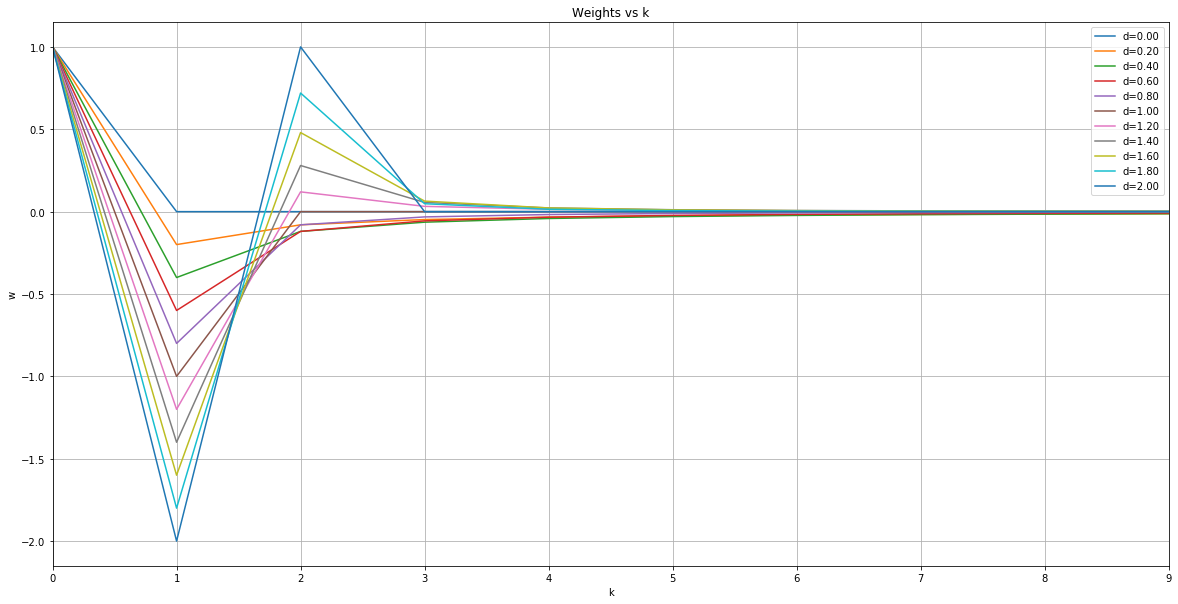
\includegraphics[width=\textwidth]{methods/images/weights_vs_k.png}
    \caption{Weight values vs. $k$ for different $d$ values.}
    \label{fig:w_k_vs_k}
\end{figure}

As it can be seen in figure \ref{fig:w_k_vs_k}, coefficients tend to zero as $k$
increases. It can also be proved the convergence of coefficients $w_k$. Let's
analyze the following when $k > d$ and $w_{k-1} \ne 0$:

\[|\frac{w_k}{w_{k-1}}| = |\frac{d-k+1}{k}| < 1 \]

what makes $|w_k| < |w_{k-1}|$ leading to $\lim_{k \to \infty} w_k = 0$.

When implementing fractional differentiation on a real time series, one has two
options:

\begin{enumerate}
  \item Adjust the length of $w_k$ vector by weight loss with a certain
        threshold.
  \item Work with a fixed number of coefficients.
\end{enumerate}

Option 1 requires the operation to compute the size of $w_k$ vector to account
for weight loss given a certain threshold. Weight loss cam be computed:

\begin{equation}
  \lambda_l = \frac{\sum_{j=T-l}^{T}|w_j|}{\sum_{i=0}^{T-1}|w_i|}
\end{equation}

where:

\begin{itemize}
  \item $T$ is the length of the time series,
  \item $l$ is the index of the sample from the end where the fractional
        differentiation occurs.
  \item $\lambda_l$ the weight loss at $l$ index
\end{itemize}

One should discard all samples whose $\lambda_l < \tau$ and $\tau$ is the
threshold. As $d \to 0$, the energy of the weights decreases leading to more
weight loss and more discarded samples.

Option 2 comes with the simplicity of having always the same vector of
coefficients $w_k$ such that $|w_k| > \tau$ and $\tau$ is a user defined
threshold. It comes with the advantage of having no drift as option 1 and just
needs to drop $l$ samples at the beginning, being $l$ the value of $l$ that
makes $w_k$ less or equal to $\tau$. In this thesis, option 2 is used.

So far, how to compute the weights vector was explained. Now, we just need to
address the value of $d$. $X_t$ might be stationary already which leads to
$d^* = 0$ with $d^*$ the value of $d$ that preserves most memory making the 
time series stationary. When $X_t$ has a \emph{unit root} (see chapter 15 of \cite{time_series_analysis}),
$0 \le d^* \leq 1$. And when $X_t$ exhibits an explosive (bubble) behavior,
$d^* > 1$. Unit roots can be tested with Dickey Fuller hypothesis test
(see chapter 17 of \cite{time_series_analysis}). The null hypothesis of the test claims the series has a unit root.
After determining a certain confidence level one can derive an \emph{optimum}
$d^*$ by:

\begin{enumerate}
  \item Define a vector of $d$ values in range of 0 to 1.
  \item For each value of $d$:
  \begin{enumerate}
    \item Fractionally differentiate $X_t$ with $d$ given a certain amount of
          weights. Obtain $X_t^d$.
    \item Compute the Dickey Fuller statistic, ADF, for $X_t^d$.
    \item Compute the p-value of the test.
  \end{enumerate}
  \item Choose $d^*$ that yields the maximum p-value between all p-values that
        are less or equal to the confidence level.
\end{enumerate}

This process has two flaws:

\begin{itemize}
  \item It is computationally time complex. Each time we apply the fractional
        differentiation, we are processing a $O(n^2)$ algorithm. Computing the
        ADF of the differentiated series requires a differentiation and model
        estimation which yields at least another $O(n^2)$ process. Finally, we
        iterate through a vector of $d$ adding another dimension.
  \item \emph{Optimum} $d$ is subject to the granularity of the $d$ vector of
        samples. The smaller the step, the more information one could preserve
        in the final time series, but the more iterations are required which
        impacts directly in the aforementioned item.
\end{itemize}

Regardless, all features that expose non-stationary characteristics could be
transformed and stabilized while preserving memory.
\subsubsection{Fundamental features}
\label{sec:methods_features_fundamental}

The dataset of bitcoin prices and volume comes with open, close, highest and
lowest daily prices, and volume expressed in transacted coins and their market
value in USD. Figures \ref{fig:btc_prices_all} and \ref{fig:btc_prices_split}
show the bitcoin daily prices. Figure \ref{fig:btc_volume} shows the volume
series.

\begin{figure}[H]
    \centering
    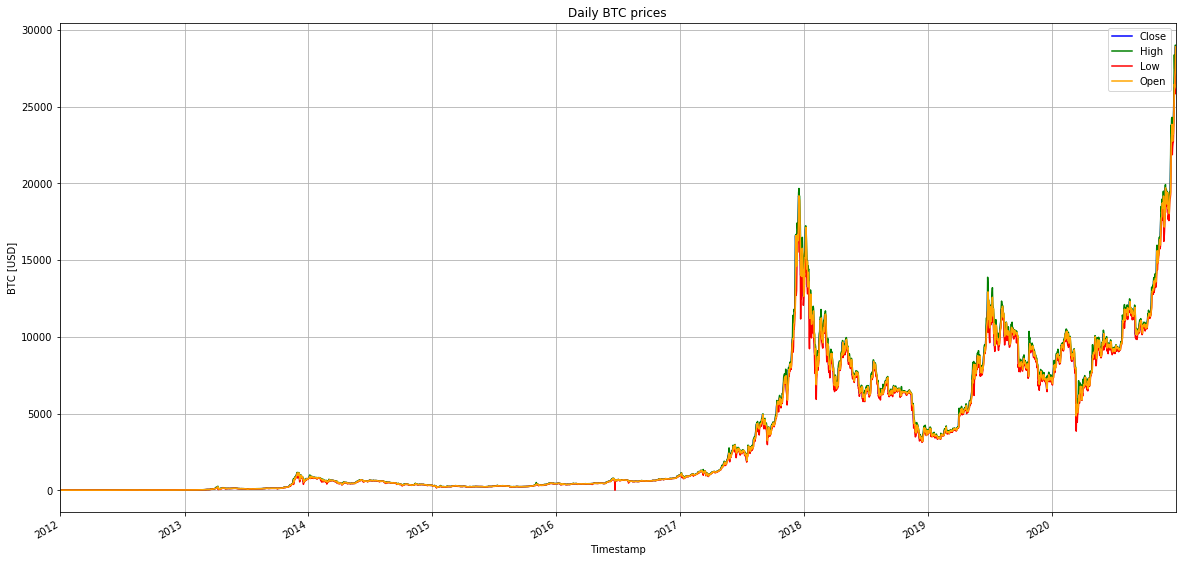
\includegraphics[width=\textwidth]{methods/images/btc_prices_all.png}
    \caption{Overlapped open, close, high and low bitcoin daily prices in USD.}
    \label{fig:btc_prices_all}
\end{figure}

\begin{figure}[H]
    \centering
    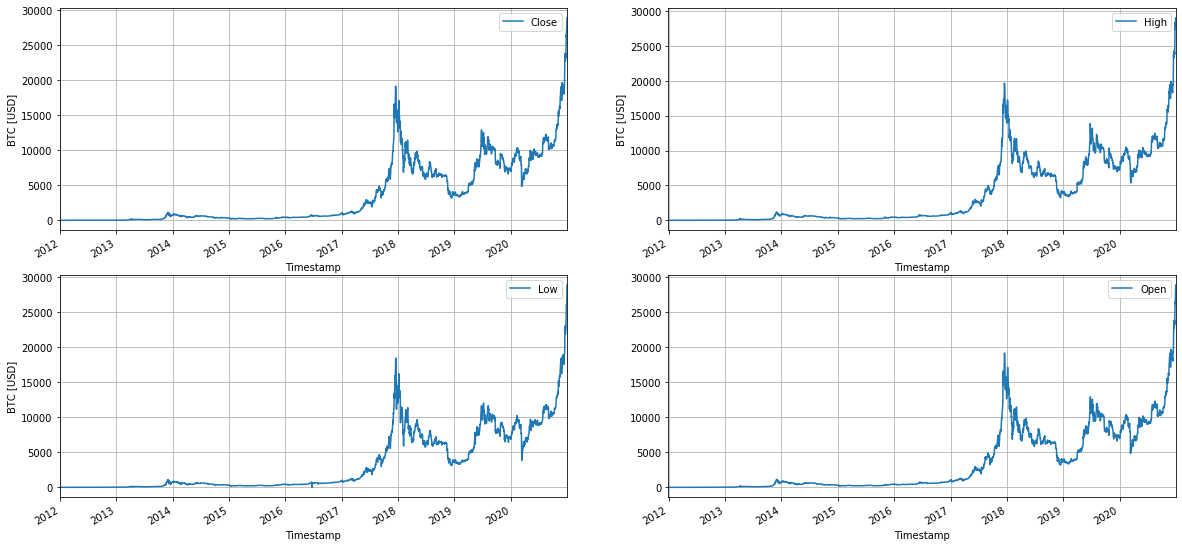
\includegraphics[width=\textwidth]{methods/images/btc_prices_split.png}
    \caption{Split of open, close, high and low bitcoin daily prices in USD.}
    \label{fig:btc_prices_split}
\end{figure}

\begin{figure}[H]
    \centering
    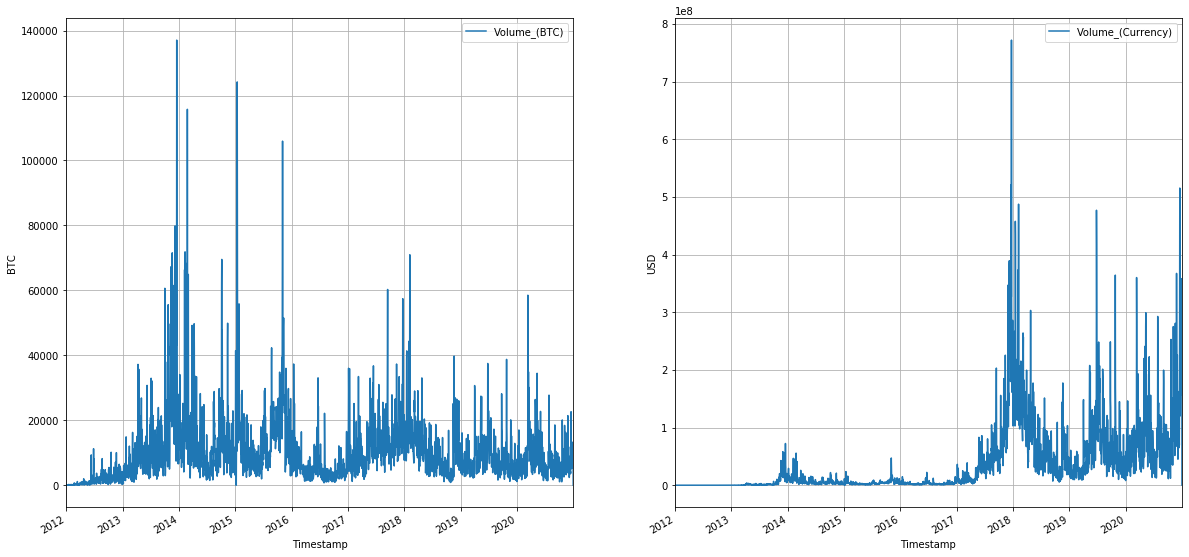
\includegraphics[width=\textwidth]{methods/images/btc_volume.png}
    \caption{The graph on the left shows the bitcoin daily volume. The graph on the right shows the market volume valuation in USD.}
    \label{fig:btc_volume}
\end{figure}

For volume series, the fractional differentiation was not enough so a log transformation
was added to stabilize the mean. Results can be seen in figure \ref{fig:btc_volume_log}.

\begin{figure}[!htb]
    \centering
    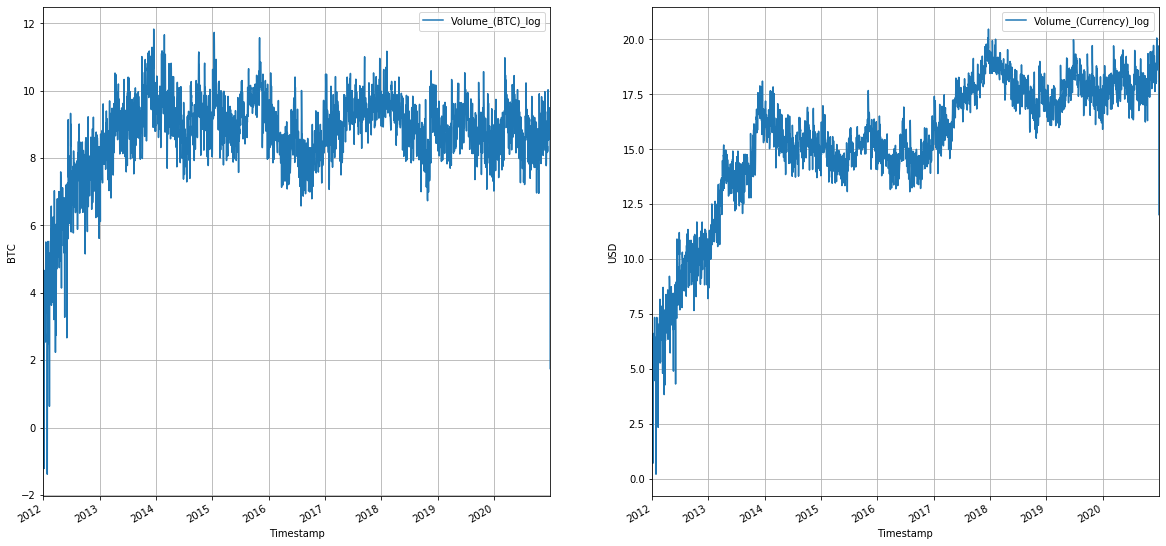
\includegraphics[width=\textwidth]{methods/images/btc_volume_log.png}
    \caption{Same features as in \ref{fig:btc_volume} but taking the logarithm.}
    \label{fig:btc_volume_log}
\end{figure}

Price series require fractional differentiation as explained in
\ref{sec:methods_features}. We could obtain the best $d^*$ for each price time
series applying the method previously described. Ten samples in the range
$[0, 1]$ are taken to look for the best $d^*$ which shields the results in table
\ref{table:frac_diff_prices}.

\begin{table}[!htb]
  \begin{center}
    \begin{tabular}{ | c | c | }
      \hline
      Feature & $d^*$ \\
      \hline
      Close   & 0.4   \\  
      \hline
      Open    & 0.4   \\
      \hline
      High    & 0.4   \\
      \hline
      Low     & 0.2   \\    
      \hline
    \end{tabular}
    \caption{Fractional differentiation order for price series.}
    \label{table:frac_diff_prices}
  \end{center}
\end{table}

Just for illustration purposes, see figure \ref{fig:close_ffd} that shows the
Close price series and the same series with an overlap of the fractionally
differentiated counterpart. Note the $y$ axis on the right which tracks the
scale of the fractionally differentiated Close price series. It can be seen
perfectly the effect of differentiating the series.

\begin{figure}[!htb]
    \centering
    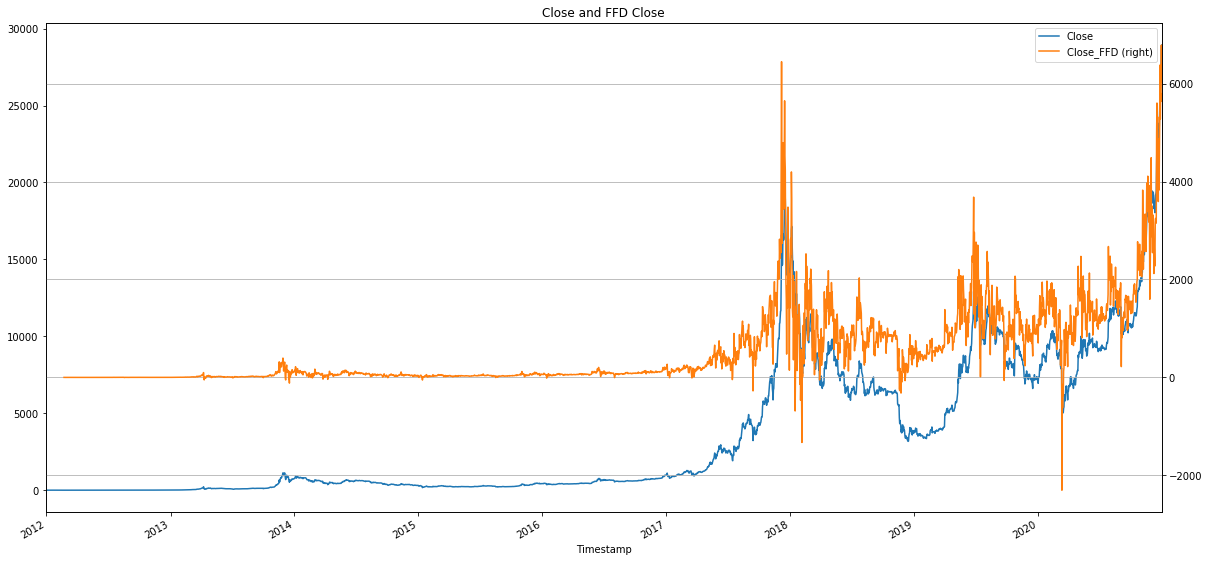
\includegraphics[width=\textwidth]{methods/images/btc_close_ffd.png}
    \caption{Close price and fractionally differentiated Close price with $d^* = 0.4$ (see table \ref{table:frac_diff_prices}).}
    \label{fig:close_ffd}
\end{figure}

On the other hand, other features were created out of the Close price series.
Those features features are:

\begin{itemize}
  \item RSI: Relative Strength Indicator. It is a momentum index that measures
        the strength or weakness of a stock price. Some time windows are used in
        favor of capturing high speed and low speed trends. See figure
        \ref{fig:rsi}.
  \item Autocorrelation: with different lags and time window lengths, the price
        series autocorrelation looks for repetitive patterns in the signal.
        Peaks in the autocorrelation signal indicate an occurrence of
        repetition. See figure \ref{fig:autocorrelation}
  \item Logarithm of the returns: just what the index expresses. It uses a
        logarithm transform to control the variance of the series. See figure
        \ref{fig:log_returns} and the histogram of values.
  \item Volatility: computed as the standard deviation of the moving average of
        the log returns. That yields the trend in return variation. Multiple
        time windows are used to capture different speeds. See figure
        \ref{fig:volatility}.
\end{itemize}

\begin{figure}[H]
    \centering
    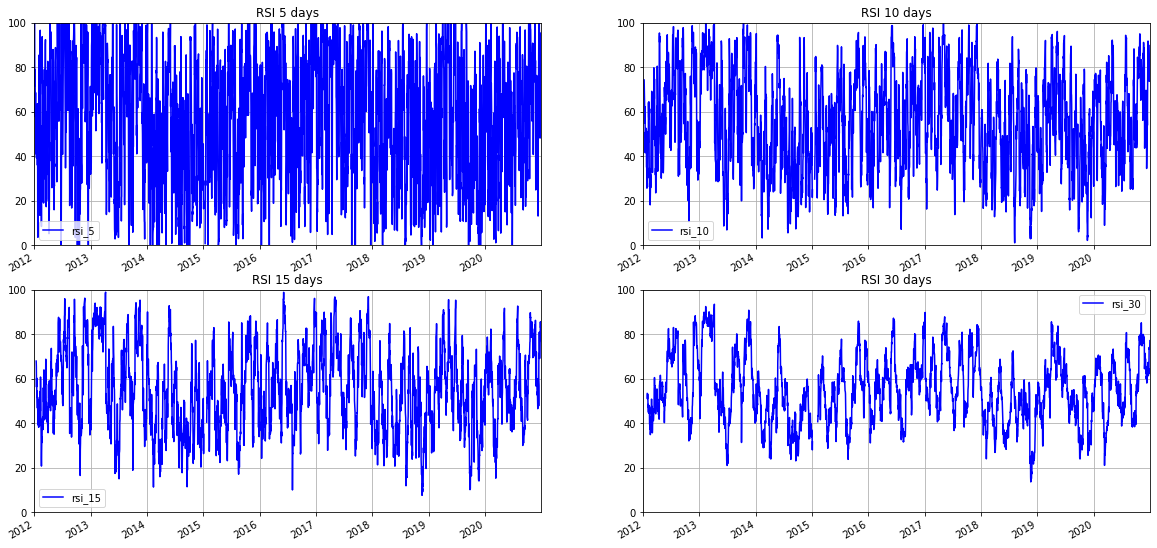
\includegraphics[width=\textwidth]{methods/images/rsi.png}
    \caption{RSI indexes for Close prices.}
    \label{fig:rsi}
\end{figure}

\begin{figure}[H]
    \centering
    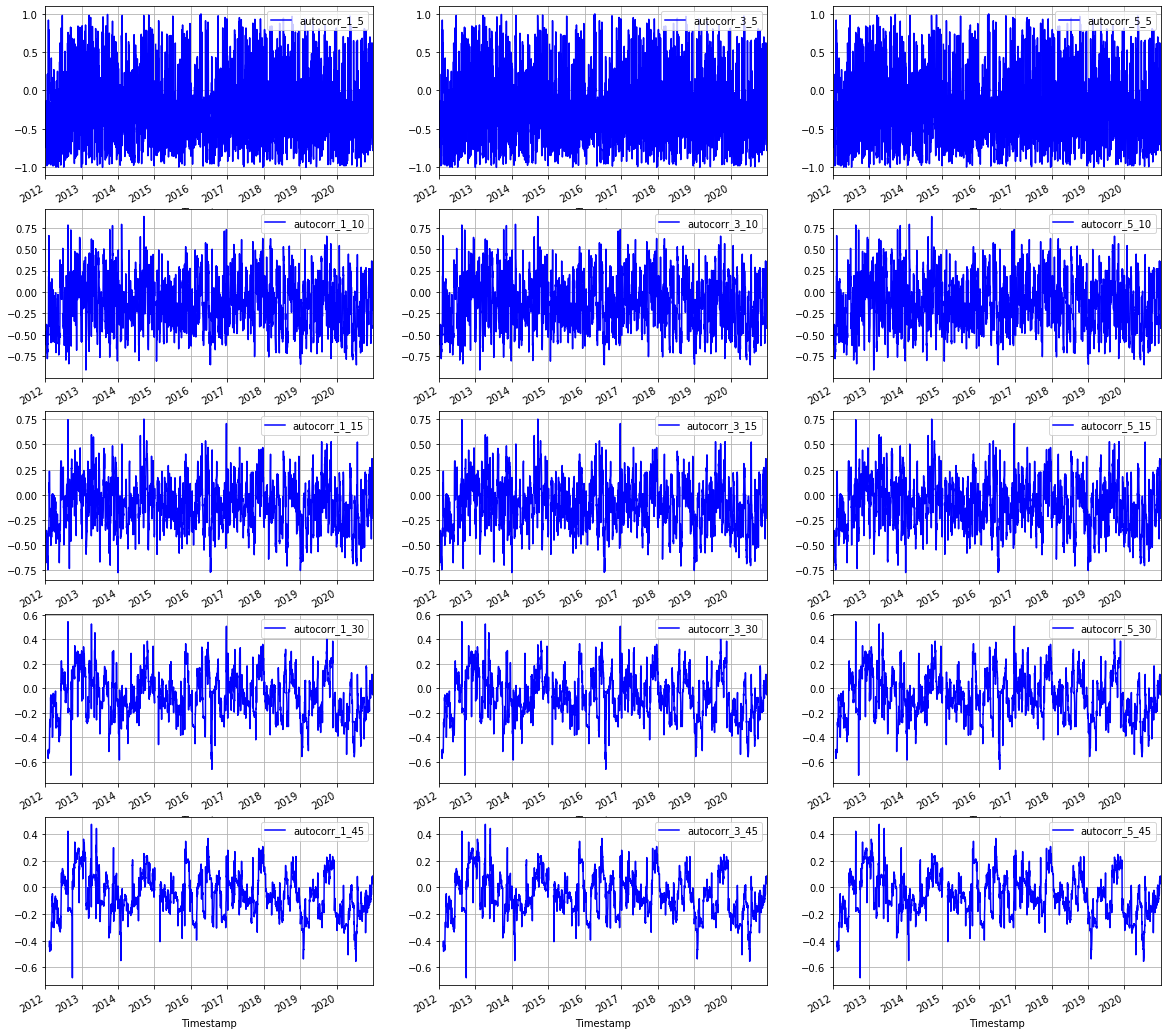
\includegraphics[width=\textwidth]{methods/images/autocorrelation.png}
    \caption{Different autocorrelation signals with different lags and time
    windows.}
    \label{fig:autocorrelation}
\end{figure}

\begin{figure}[H]
    \centering
    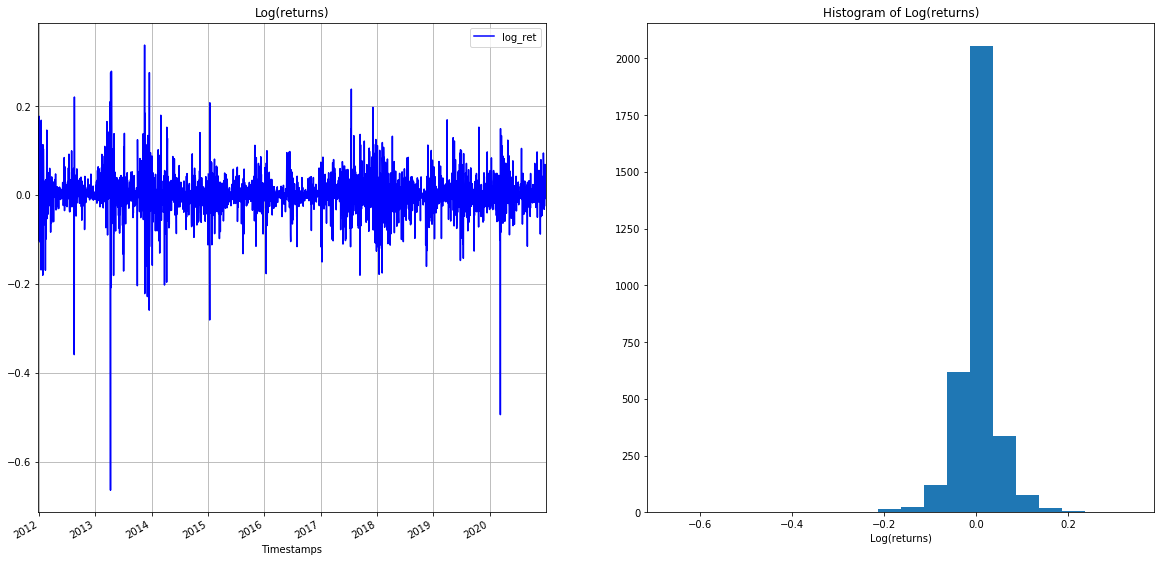
\includegraphics[width=\textwidth]{methods/images/log_returns.png}
    \caption{Logarithm of returns on the left, the histogram of the logarithm of returns on the right.}
    \label{fig:log_returns}
\end{figure}

\begin{figure}[H]
    \centering
    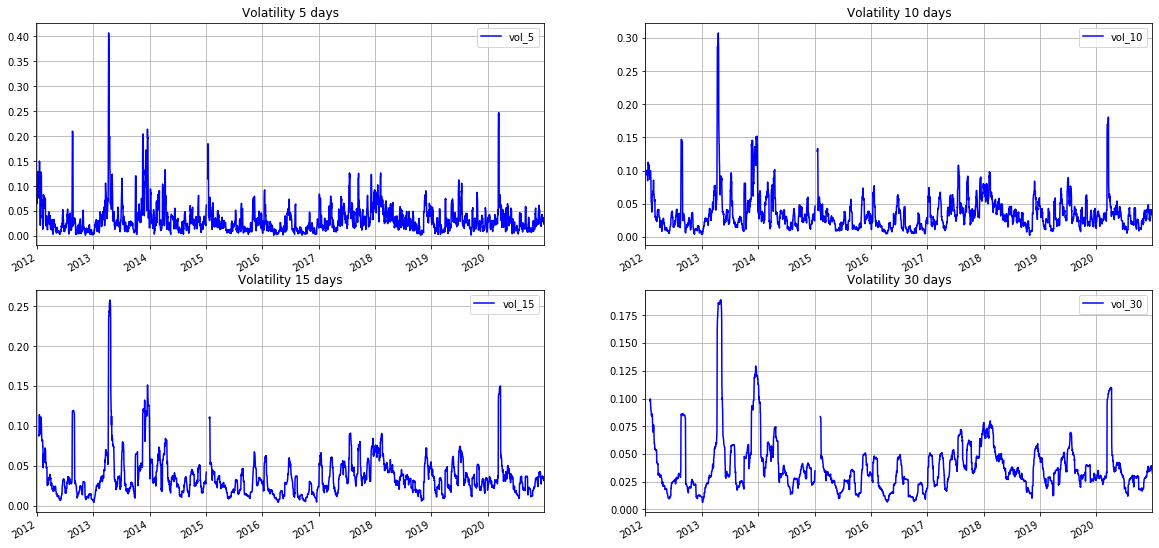
\includegraphics[width=\textwidth]{methods/images/volatility.png}
    \caption{Volatility index.}
    \label{fig:volatility}
\end{figure}
\subsection{Domain}
\label{sec:intro_domain}

This section outlines the theoretical background of each related knowledge domain involved in this research. The following list introduces each subsection:

\begin{itemize}
    \item Subsection \ref{sec:intro_fundamental_trading_strategies} describes the primary model which is a momentum strategy and why it was chosen.
    \item Subsection \ref{sec:intro_crypto_currencies} provides background about cryptoassets, cryptocurrencies and in particular Bitcoin and its ecosystem.
    \item Subsection \ref{sec:intro_financial_machine_learning} introduces the methodology Lopez de Prado explains in \cite{lopez_de_prado}, answers why machine learning is applied and introduces the structure break indexes with strong focus on SADF.
\end{itemize}

As detailed in \ref{sec:intro_problem_description}, the research problem involves many knowledge domains and data from different sources. When working in finance, models need to account for the independent variable time as markets \emph{evolve} with it, i.e. they are dynamic. Among all the available strategies to derive the primary model, momentum was chosen.

\subsubsection{Fundamental trading strategies}
\label{sec:intro_fundamental_trading_strategies}

There are many algorithmic fundamental trading strategies. We can use the classification in \cite{oxford_handbook}:

\begin{itemize}
    \item Impact driven: orders placed in a market affect the price of the stocks based on their volume and the liquidity. Strategies like volume-weighted average price (VWAP) or time-weighted average price (TWAP) can be found in this group.
    \item Cost driven: it not only considers implicit costs as the above but also the explicit costs of the market (e.g. commissions and access fees). We can find implementation shortfall in this group.
    \item Newsreader: based on the semi-strong form efficiency, these algorithms exploit news feeds to derive trading signals out of non-structured data.
    \item Market making: this group exploits the spread in the bid-ask prices.
    \item Statistical arbitrage: strategies in this group focus on two main premises: an asset tends to a \emph{medium} value in the long run (one can profit from deviations) or an asset's price is nonstationary, i.e. it fluctuates without a central value (one can profit from the tendency estimation). Mean reversion and momentum strategies belong to this group.
\end{itemize}

Momentum based strategies focus on deriving when a price starts to rise and drop to derive signals and profit by placing long and short positions on the asset. To derive these events, two different speed (fast and slow) moving average signals are used. The specific timestamps at which the fast and slow averaged signals cross determine an event. A fast signal crossing above the slow signal generates a buy event and the opposite generates a sell signal. A simple variation involves using exponential moving averages instead of simple moving averages and it increase complexity to even entire portfolios behind ETFs like MTUM (\cite{mtum_etf}).

In \cite{value_momentum} the authors explored the performance of momentum with market information of more than 200 years and confirm the strategy generally outperforms the market. In \cite{fact_fiction_momentum} the strategy is demystified in favor of a better comprehension of its strong and weak points. Based on the extensive literature around this strategy in particular, implementation simplicity, compatibility with the available data (no book order available, just stamped prices and volumes) this strategy was chosen to work as primary model.

\subsubsection{Cryptocurrencies}
\label{sec:intro_crypto_currencies}

Satoshi Nakamoto published \cite{bitcoin} with the intention to kick start a decentralized peer-to-peer cash system. However, it did not only do that but also gave birth to a new technology hype which is in continuous evolution and now is heading to mature the stack of services on top of the blockchain technology (\cite{deloitte}).

Let me present a few useful definitions:

\begin{itemize}
    \item Bitcoin: is the software that facilitates the transfer and custody of the bitcoin currency.
    \item bitcoin: a cryptocurrency.
    \item Blockchain: is a transaction database, in this case of the Bitcoin software. It keeps track of all debits and credits of bitcoin applying a very clever and sophisticated fashion (see  \cite{blockchain} for a comprehensive description). 
\end{itemize}

Bitcoin's blockchain technology provides several features:

\begin{itemize}
    \item It is publicly distributed. There are no secrete transactions.
    \item Serves as a historical record of \emph{all} transactions.
    \item It is immutable. Transactions will only be appended in the shape of new information blocks, but the \emph{verified} past cannot be changed.
    \item It is secure, i.e. each transaction is cryptographically verified to ensure valid funds. 
\end{itemize}

Transactions are verified via a \emph{Proof-of-Work} (PoW) algorithm which requires nowadays specialized hardware to process the cryptographic algorithm in a timely and competitive manner. Timely and competitive go hand in hand because the first \emph{miner} in claiming the block hash (result of the PoW) obtains a bitcoin reward provided by the Bitcoin software. The block hash is expensive to obtain but easy to verify what makes the acceptance of a new block a fast process for the entire network.

So far, we have introduced some of the technical characteristics of Bitcoin and supporting technologies. It is important to mention what this payment network provides to users. On one hand we have the privacy. Transactions happen from one wallet \cite{wallet} to another (cryptography comes in to properly describe how they work which is out of the scope of this document) and there is no direct nor easy way to know how is the owner of the wallet. Simply, there is information record about the owner of the wallet operation other than the transaction ledger (the blockchain itself). On the other hand, Bitcoin runs on the internet (using TCP \cite{bitcoin_network}) even on countries with network traffic control which sets the basis to trade worldwide without any regulation.

Another important aspect about bitcoin is the issuance model. Miners are paid every time they append a new block and receive a reward in bitcoins. The reward was initially set to 50 bitcoins and Bitcoin would adjust the mining complexity to get a new block every ten minutes on average. On a 210,000 blocks basis, the reward gets reduced to a half although the complexity keeps on adjusting to have the same throughput of one block every ten minutes. The total amount of bitcoins to be issued is 21 million and we can see in figure \ref{fig:issued_bitcoins} the amount of bitcoins issued by April 2020.

\begin{figure}[!htb]
    \centering
    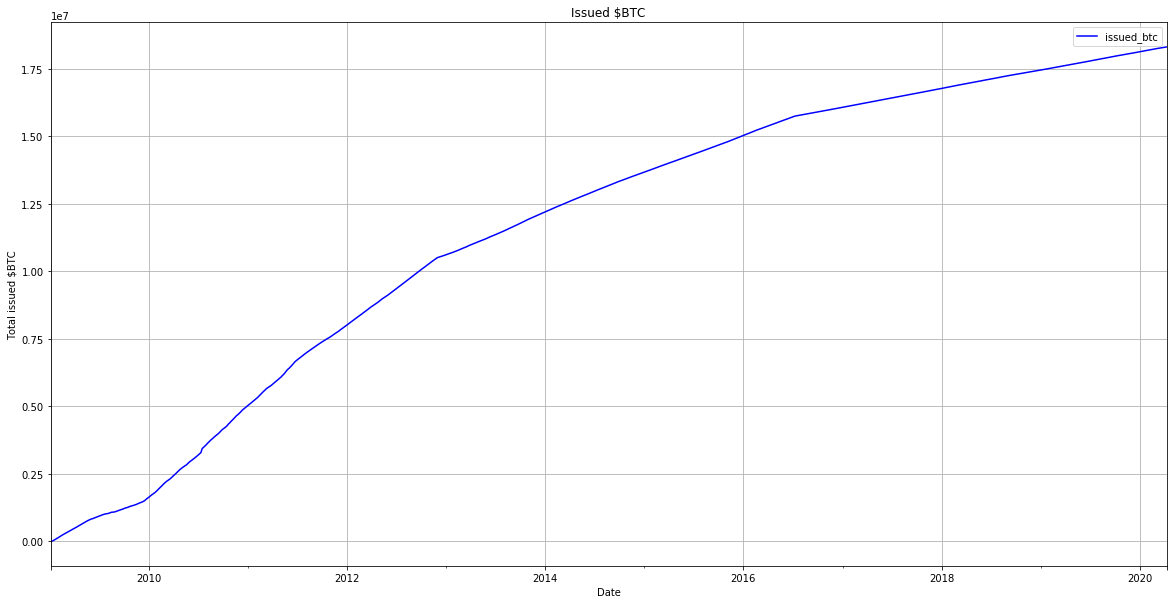
\includegraphics[width=\textwidth]{introduction/images/issued_btc.png}
    \caption{Issued bitcoins through time. Vertical scale is in tenths of millions of bitcoins. Glassnode data.}
    \label{fig:issued_bitcoins}
\end{figure}

And in \ref{fig:issuance} we can see the evolution of bitcoin issuance with time. By April 2021, the total amount of issued bitcoins is 18.66 millions roughly a 88.9\% of the 21 million.

\begin{figure}[!htb]
    \centering
    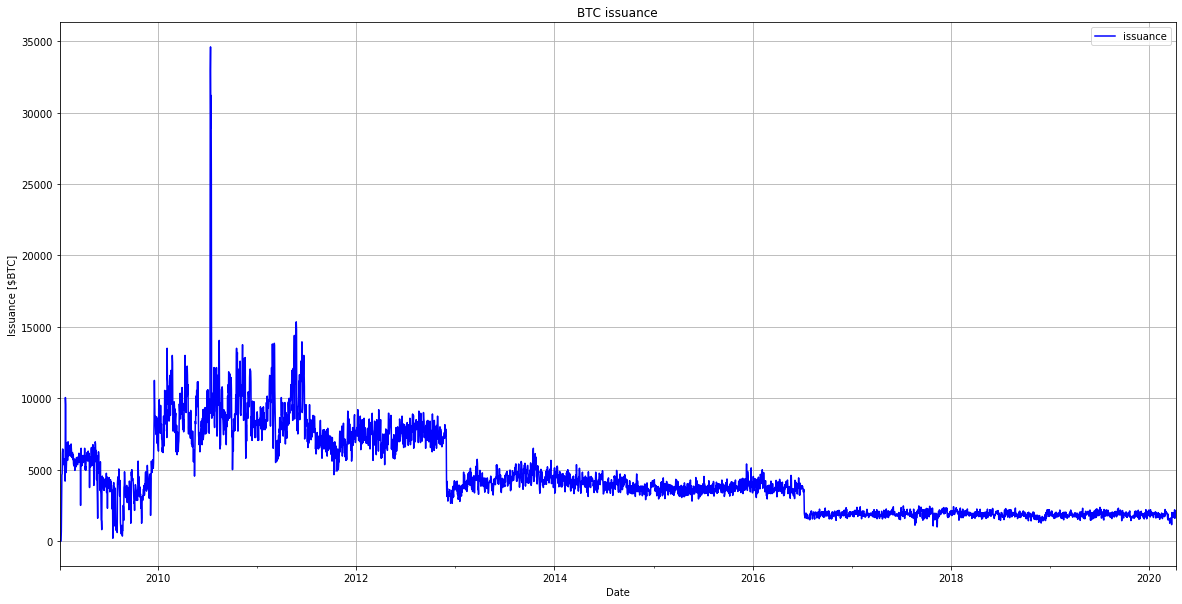
\includegraphics[width=\textwidth]{introduction/images/issuance.png}
    \caption{Bitcoin issuance through time. Glassnode data.}
    \label{fig:issuance}
\end{figure}

As it could be seen in \ref{fig:issuance} and in  \ref{fig:issued_bitcoins} the total number of bitcoins is decelerating. By design, bitcoin is a scarce asset. In \cite{bitcoin_stock_to_flow}, PlanB suggests to use a stock to flow (S/F) model to estimate the value of bitcoin scarcity. In figure \ref{fig:stock_to_flow} the close price series and the S/F ratio are shown to better explain its correlation. In blue we can see the how S/F ratio varies with time and in green we see the close price of bitcoin (note the vertical axis is plotted using a logarithmic scale). In red dotted vertical lines we see the days of the halvings (on 2012/11/28, 2016/07/09, and 2020/05/11). Along this feature (S/F ratio) others will be used that are very specific of the Bitcoin infrastructure and technology. Refer to \ref{sec:material_data_bitcoin_features} for a comprehensive description of the features.

\begin{figure}[!htb]
    \centering
    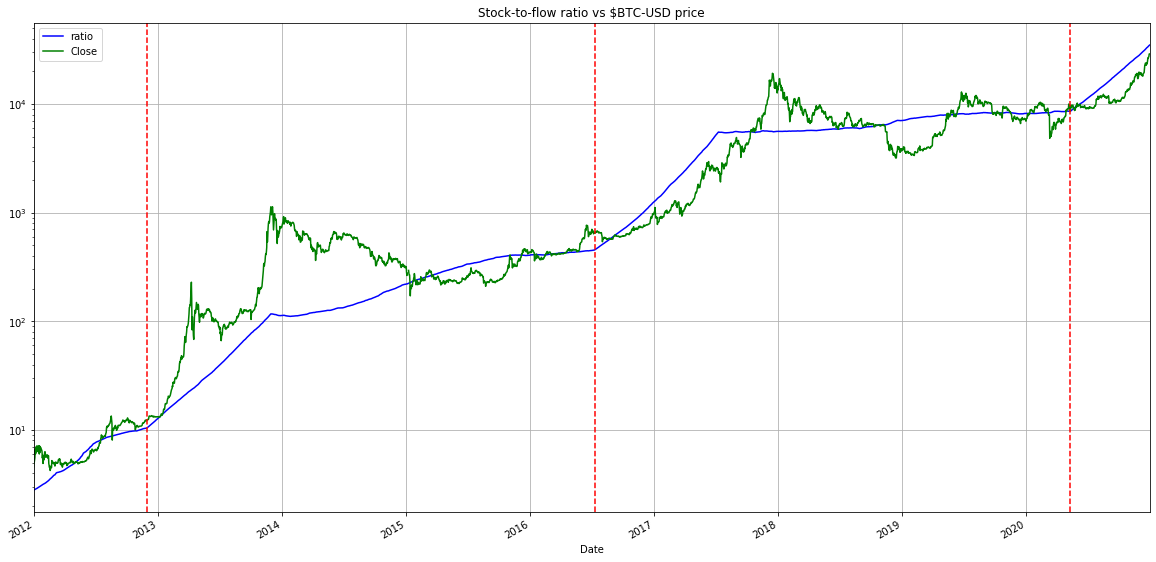
\includegraphics[width=\textwidth]{introduction/images/stock-to-flow.png}
    \caption{S/F ratio versus the close daily price in USD. Plotted in logarithmic vertical scale.}
    \label{fig:stock_to_flow}
\end{figure}

After Bitcoin software was released and gained attraction from different communities, other projects were created \emph{from} it (e.g. the so-called \emph{forks}). Bitcoin is an open source software project (\cite{bitcoin_github}) with a compatible license for both private and public usage which enabled people all around the world to use this technology for multiple purposes such as promotion of new bitcoin-like coins, projects running on top of the blockchain technology, etc.

In this research project we will use bitcoin: the top cryptocurrency by market capitalization as of April 2021 and the first cryptocurrency which started a revolution.

\subsubsection{Financial machine learning}
\label{sec:intro_financial_machine_learning}

This research project involves applied machine learning to finance where it is specifically applied to a trading strategy to learn the size of the position at each bet. In \cite{lopez_de_prado} it is described the procedure to properly develop a machine learning pipeline for a financial application like this one. Lopez de Prado described in \cite{future_of_empirical_finance} problems in financial research publications. The author relates those problems to bad practices and practitioners' ethics sometimes but he also recommended ways to mitigate those issues and their consequences. We could find a similar approach in \cite{lopez_de_prado} with a more in deep explanation of all the aspects which attain the machine learning pipeline to develop.  

As stated before, in this research project we will develop a strategy based on momentum to determine when and how (long vs. short) place our positions. That would define our primary model which follows a secondary model (the machine learning model) to derive the size of the position. Sizing the bet is a two step process: first  we obtain the probability that the buy or sell signal is accurate and second we compute the size of the the bet out of the probability. The model used to derive the probability could be a logistic regression, a tree based model, a neural network, a SVM or whatever model the researcher considers and \emph{finds} that yields better \emph{results}. This research project will focus on comparing some tree based models and evaluating based on \cite{lopez_de_prado} recommendations to mitigate common flaws that will certainly derive into runtime strategy biases and, consequently, losses.

In preparation to train the model, the well known feature engineering stage will be performed. In this case, univariate, bivariate, scaling and other techniques (\cite{feature_engineering}) are relevant but not enough. At least two chapters of \cite{lopez_de_prado} workout in detail two aspect of the time series analysis from a feature point of view: sample uniqueness (explained in section \ref{sec:methods_pipeline_secondary_model}) and sample stationarity (see chapter 15 \cite{time_series_analysis}) vs. loss of memory dilemma (explained in detail in section \ref{sec:methods_features}). One can find thorough explanations of the effects of bootstrap sampling and their effects on the model error (see section 7.11 of \cite{elements_of_statistical_learning}) but it does not usually consider the \emph{duration} of a sample because those in the dataset are often considered both independent and identically distributed (IID) as well as without duration. This is not the case of financial events like this one. Two or more \emph{signals} might overlap due to high volatility in the market or to correlated information. If the model does not take into account that those \emph{signals} refer to the same unique \emph{event} we would incur in unbalanced datasets when training a model due to variations in \emph{event} representativeness. On the other hand, to perform inference we require signals to be stationary but that comes at the expense of removing memory which is essential to obtain the predictive power. Lopez de Prado proposes to use fractional differentiation (see \cite{frac_diff_paper} for the possibly first known occurrence of the method) to determine the minimum differentiation factor $d$ such that the non stationarity null hypothesis of the series is rejected. Hence, some memory will remain in the series and the model can benefit from it.

\begin{figure}[!htb]
    \centering
    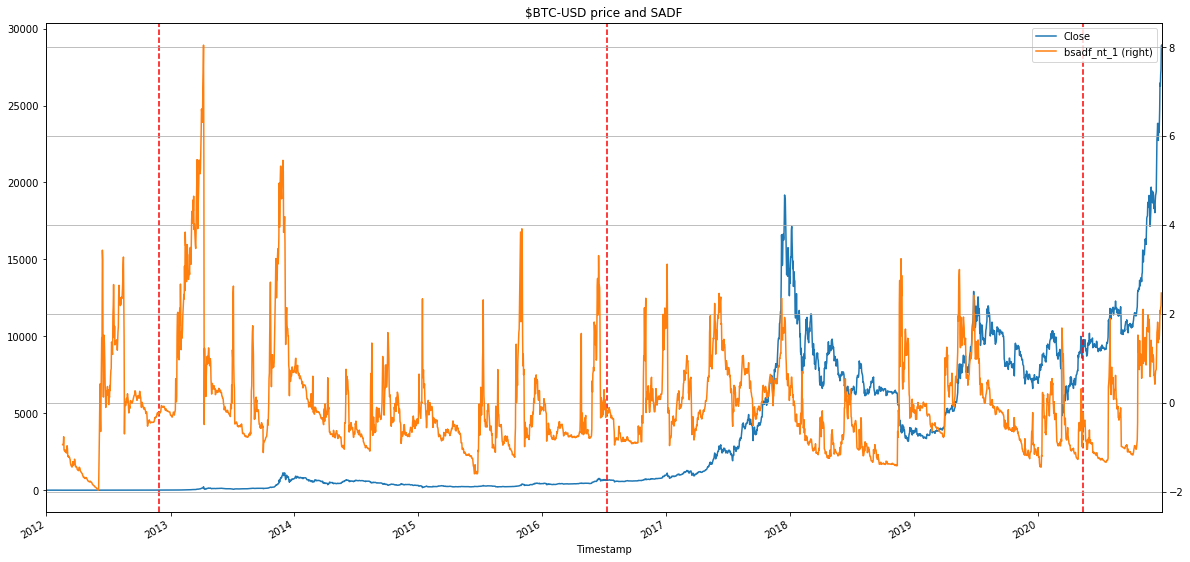
\includegraphics[width=\textwidth]{introduction/images/sadf_vs_price.png}
    \caption{Bitcoin price evolution and SADF index.}
    \label{fig:sadf_vs_price}
\end{figure}

\begin{figure}[!htb]
    \centering
    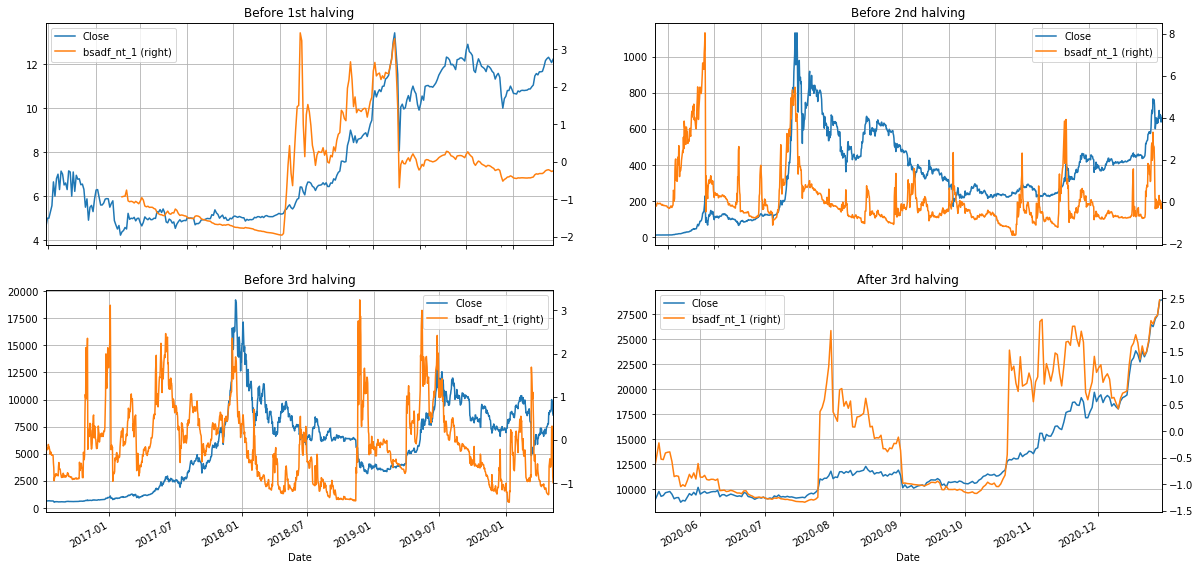
\includegraphics[width=\textwidth]{introduction/images/sadf_per_period.png}
    \caption{Bitcoin price evolution and SADF index by issuance period.}
    \label{fig:sadf_by_halving}
\end{figure}

In \ref{sec:intro_crypto_currencies}, the Stock to Flow model and halvings were introduced. The scarcity model and the issuance scheme imply regime breaks in the price series. Those events are called \emph{structural breaks} and specific features can be built to provide prediction power to our models, see \ref{sec:methods_features_sadf}. In chapter 17 of \cite{lopez_de_prado}, the author classifies into four the types of structural break tests: CUSUM tests, explosiveness tests, right-tail unit-root tests and sub/super-martingale tests. One can find within the explosiveness tests the Supremum Augmented Dickey-Fuller test (SADF, \cite{sadf_paper}) which evaluates successive bubble-like behaviors. The core idea of the index is that the price follows a random walk series and at some point it becomes an explosive test which ends up in a bubble burst. This process could repeat. The SADF index would raise when the bubble is growing and drastically decrease when the bubble explodes. Figure \ref{fig:sadf_vs_price} shows the evolution of the index over the prices. It is not trivial to see the relevance of this index unless we partition the price series by halvings and see it in figure \ref{fig:sadf_by_halving}.


Moreover, cross validation for training will be discussed and some tweaks we can use to improve the training technique as well as which model metrics we should use to compare machine learning models. Once all the features and the pipeline to train the model is in place, dimensionality reduction by feature selection will be applied to reduce the amount of required data while preserving model performance. Here, different methods will be compared in favor of increased decision robustness. Finally, backtesting of the strategy will be performed with strong emphasis on the the methodology.

\subsubsection{Supremum Augmented Dickey Fuller}
\label{sec:methods_features_sadf}

Section \ref{sec:intro_domain} briefly introduced the concept of structural
breaks and the index to be implemented and used in this research project, SADF.
In words of Lopez de Prado:

\say{In developing an ML-based investment strategy, we typically wish to bet
when there is a confluence of factors whose predicted outcome offers a favorable
risk-adjusted return. Structural breaks, like transition from one market regime
to another, is one example of particular interest.}

The problem appears when trying to quantitatively detect how a regime change
occurs. In \cite{sadf_paper} Phillips, Wu and Yu studied Nasdaq index in 1990
prior to the famous DotCom bubble and proposed a new index based on recursive 
augmented Dickey-Fuller tests for unit root against the alternative of an
explosive root (the right-tailed). The objective of this test is to identify
the presence of exponential growth or collapse, while assuming an autoregressive
specification.

In price series, like the one used in this research project, not only
one, but many bubbles are prune to happen. Not all indexes are useful under this
assumption as many fail to detect recurrent bubbles. Nevertheless, we will start
analyzing the case of just one bubble in the series and then generalize it to
many as the it is described in chapter 17 of \cite{lopez_de_prado}. Suppose a
price series that follows a first order autoregressive process:

\[ y_{t} = \rho y_{t-1} + \epsilon_{t} \]

where $\epsilon_{t} \sim N(0, \sigma_{y}^{2})$, i.e. white noise. We can create a
test to evaluate the value of $\rho$ whose null hypothesis states that the price
series follows a random walk. In other words, $H_{0}: \rho = 1$ and the
alternative hypothesis is that $y_t$ starts as a random walk but at some point
in time $t^{*}T$ the process becomes explosive, such:

\begin{equation}
  H_{1} :
    \begin{cases}
      \rho = 1 & \text{if t = 1, ..., $\tau^{*}T$}\\
      \rho > 1 & \text{if t = $\tau^{*}T$, ..., T}\\
    \end{cases}       
\end{equation}

where $\tau^{*} \in (0,1)$. At the end of the series, i.e. at $T$, one
could try to find the value $\tau^{*}$ where there was a change of regime from
random walk to an explosive process. To test this hypothesis, we should
consider:

\[ \Delta y_{t} = \delta y_{t-1} D_t[\tau^{*}] + \epsilon_{t}\]

where $D_t[\tau^{*}]$ is a dummy variable that takes the value of 0 when
$t < \tau^{*}T$ and 1 otherwise. $H_{0}: \delta = 0$ which is tested against the
one-sided alternative $H_{1}: \delta > 1$ leading to an statistic:

\[ DFC_{\tau^{*}} = \frac{\hat{\delta}}{\hat{\sigma}_{\delta}} \]

One needs to determine the value of $\tau^{*}$ because it is unknown. The
approach to determine it is to compute the supremum statistic for each possible
value of $\tau^{*}$ in the series. That would determine the start of the explosive
process yielding to a bubble. Note that only the beginning of the regime change
is determined with this method, i.e. there is no return to a random walk after
the bubble starts. This is where the novelty of Phillips, Wu and Yu appears by
a few key differences to the autoregressive model and test:

\begin{itemize}
  \item The regression specification becomes: $ \Delta y_t = \alpha + \beta y_{t-1} + \sum_{l=1}^{L} \gamma_{l} \Delta y_{t-l} + \epsilon_t$
  \item $H_{0}: \beta \le 0$, and $H_{1}: \beta > 0$
  \item $SADF_t = \sup_{t_{0} \in [1, t-\tau]} \{ADF_{t_{0},t}\} = \sup_{t_{0} \in [1, t-\tau]} \frac{\hat{\beta}_{t_{0},t}}{\hat{\sigma}_{\beta_{0},t}}$
\end{itemize}

A few differences with respect to the original, one-bubble model can be noted:

\begin{itemize}
  \item The regression is changed, there is no more a dummy $D_t[\tau^{*}]$
        variable. Instead, the regression starts at $t_{0} \in [1, t-\tau]$ and
        ends in $t \in [\tau, T]$.
  \item $SADF_t$ computes the supremum in a double nested loop for every
        possible value of $t_0$ and $t$ which are the indexes to segment the
        series.
\end{itemize}

The aforementioned characteristics allows SADF to vary provided that it is not
computed just for one time ($T$), but instead for many (every value of
$t \in [\tau, T]$).

Getting into the details of the augmented Dickey-Fuller statistic, the
confidence value should be set from the sample to yield the best results. In
\cite{sadf_paper} the authors refer to a value close to 4\% to deliver the best
performance but values between 1\% and 5\% are recommended. 5\% was used in this
case.

\paragraph{Implementation notes:} Lopez de Prado offers in his book almost
the entire algorithm (see chapter 17 of \cite{lopez_de_prado}), but leaves
behind the outer loop which allows to move forward the $SADF_{t}$ for each
$t \in [\tau, T]$. A modification was introduced in code to avoid excessive and
inefficient computation in the inner loop: an upper bound for the window was
introduced to so that the range of $t$ becomes $[max(\tau, t - \Delta t_{max}), T]$.
Although the asymptotic computational complexity of this series generation is
high ($O(n^5)$ at least, see \cite{lopez_de_prado} for a detailed analysis), one
way to saturate one order is to use $\Delta t_{max}$ which should be cautiously
selected to account for long lasting bubbles.

On a separate note, the algorithm allows researchers to introduce a constant, a
linear and a quadratic polynomial regression depending on the type of series to
analyze. All of them were computed in favor of feeding the model with more data
and experiment what yields the best results.

Finally, a recommendation in the article \cite{sadf_paper} and discussed in
\cite{lopez_de_prado} has been implemented. Instead of using raw prices, the
algorithm takes as input log-prices. Conceptually, by applying the logarithmic
transformation, the variance of the process gets stabilized and the
heteroscedastic assumption about the data can be fulfilled. Long time series
are expected to change their price levels but that does not directly cause a
regime change and the transformation facilitates to distinguish them. A regime
change implies a transition to an explosive behavior, e.g. exponential behavior
is identified.

Three pictures are shown to illustrate this index: \ref{fig:sadf_prices},
\ref{fig:sadf_prices_ffd}, and \ref{fig:sadf_prices_log}. They contrast the
index with raw bitcoin close price, fractionally differentiated bitcoin price
and log prices respectively. Note the progression in the pictures and how the 
volatility of the log-prices series correlates with SADF spikes
\ref{fig:sadf_prices_log}.

\begin{figure}[H]
    \centering
    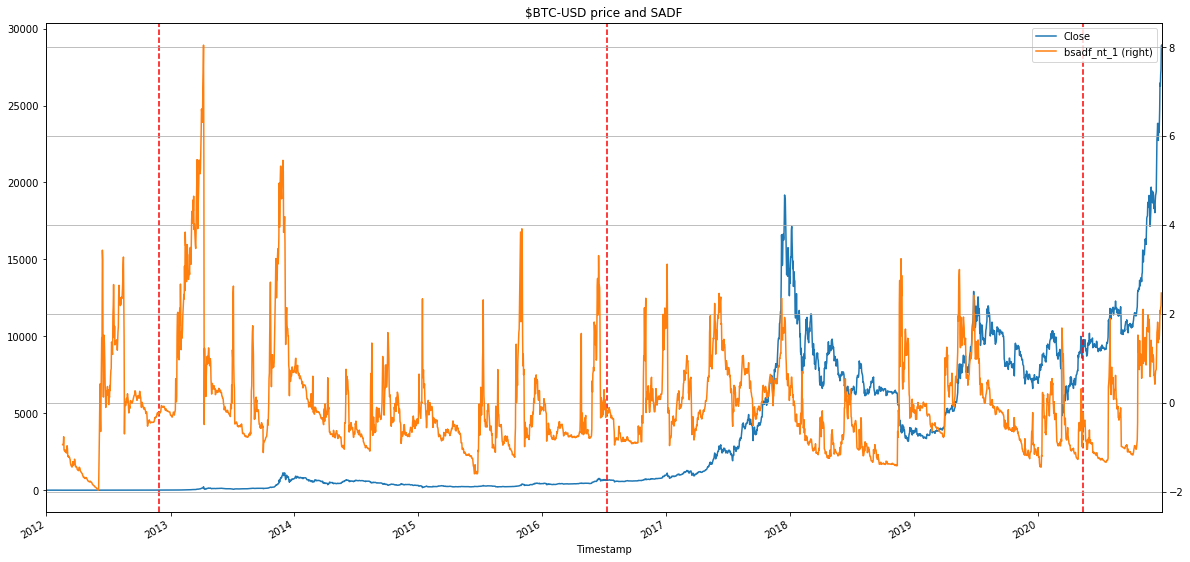
\includegraphics[width=\textwidth]{methods/images/sadf_prices.png}
    \caption{Raw close prices and SADF over time.}
    \label{fig:sadf_prices}
\end{figure}

\begin{figure}[H]
    \centering
    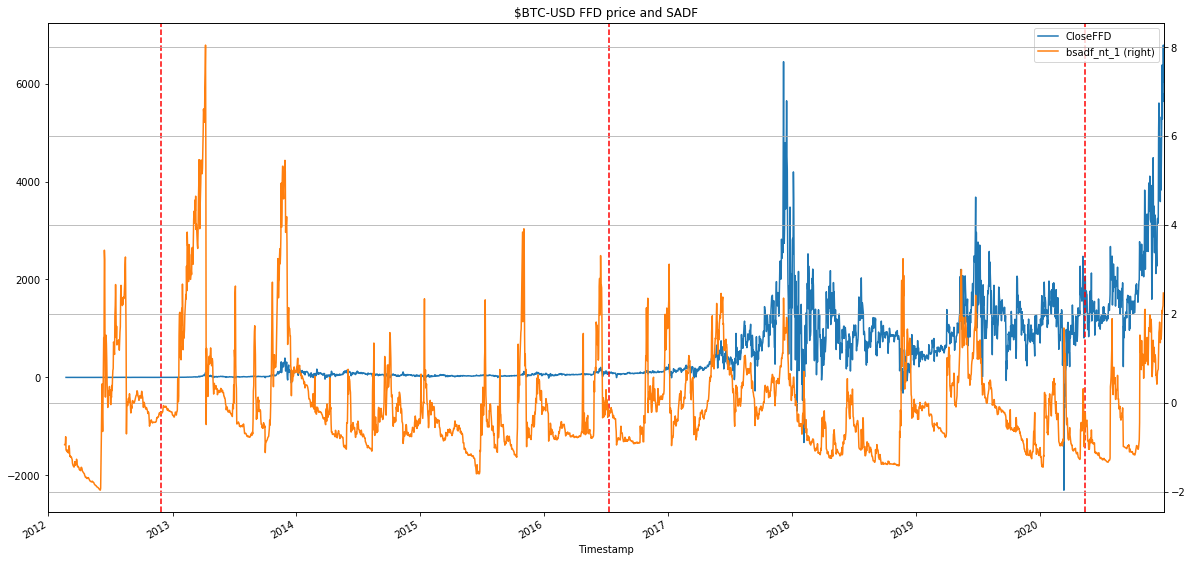
\includegraphics[width=\textwidth]{methods/images/sadf_prices_ffd.png}
    \caption{Fractionally differentiated prices and SADF over time.}
    \label{fig:sadf_prices_ffd}
\end{figure}

\begin{figure}[H]
    \centering
    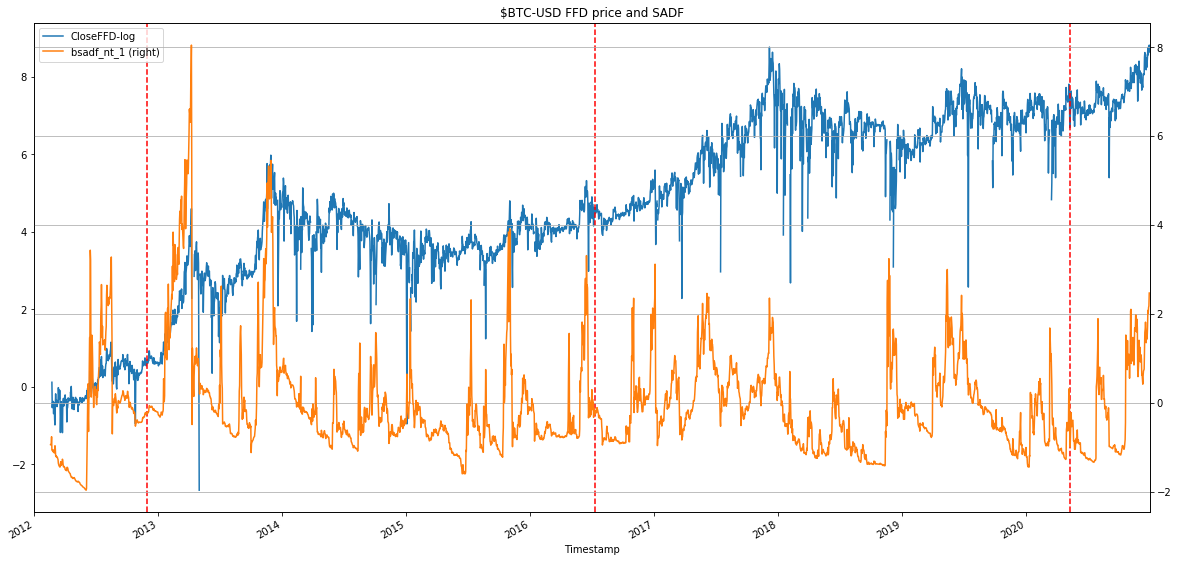
\includegraphics[width=\textwidth]{methods/images/sadf_prices_log.png}
    \caption{Close log-prices and SADF over time.}
    \label{fig:sadf_prices_log}
\end{figure}


\subsubsection{Social features}
\label{sec:methods_features_social}

So far, there were explained traditional financial features, then Bitcoin and
bitcoin features, and finally structural break features to introduce SADF
computation. Nevertheless, nothing has been said about the agents that operate
in this market so far. Therefore, what follows shows some figures to illustrate
the data gathered from the two sources: Google Trends and
Alternative.me.

First, in figure \ref{fig:google_trends} the bitcoin price series is shown
together with the interest index that Google Trends offers. Note that a linear
interpolation was used to fit daily values because social data was available
only a weekly basis. We can see that there is a better fit between the curve
shapes in the third regime and after the third halving on.

Finally, in figure \ref{fig:alternative_me} the sentiment index is displayed
for the last two periods. Data for the first two two periods was not available.
It is worth mentioning that this series is the result of fused data from
Twitter, Reddit and other forums which is definitely richer than Google Trends
interest index. Google Trends is just used to compensate social information
during the first two periods.

\begin{figure}[H]
    \centering
    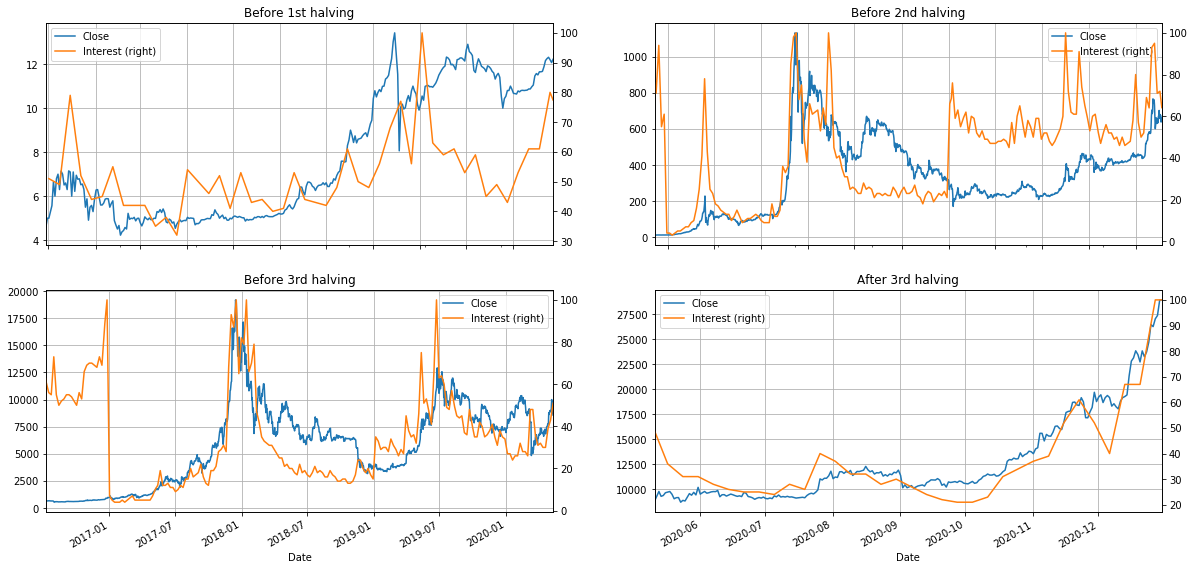
\includegraphics[width=\textwidth]{methods/images/gtrends_price_per_halving.png}
    \caption{Evolution over each bitcoin regime of the Google Trends interest in the "bitcoin" keyword together with the close price of bitcoin.}
    \label{fig:google_trends}
\end{figure}

\begin{figure}[H]
    \centering
    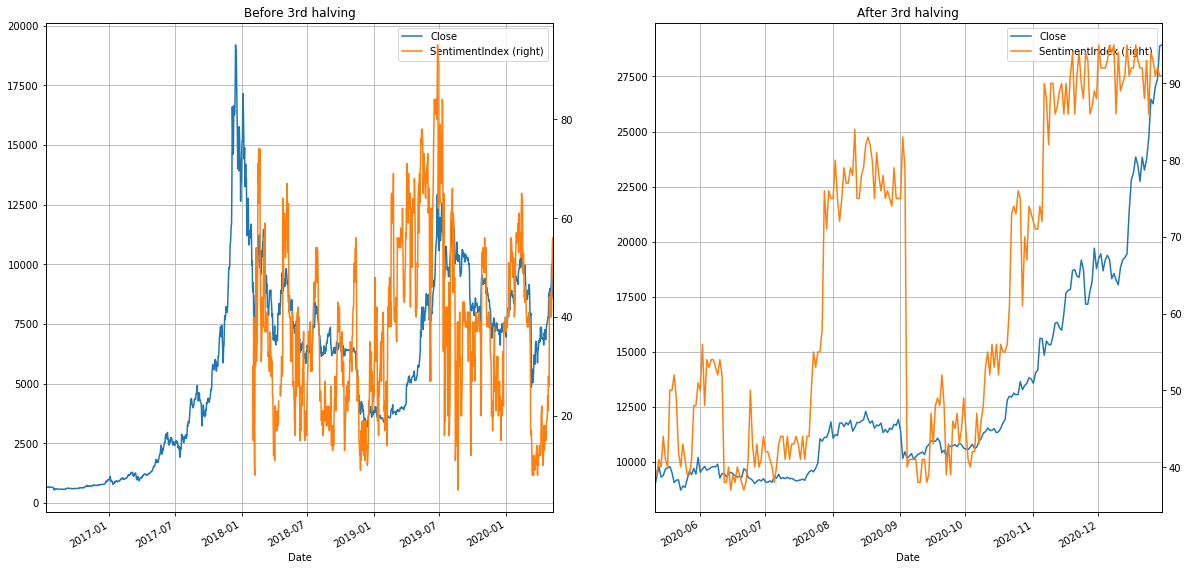
\includegraphics[width=\textwidth]{methods/images/alternative_me_halvings.png}
    \caption{Evolution over the last two bitcoin's regimes of the Alternative.me social interest of bitcoin together with the close price of bitcoin.}
    \label{fig:alternative_me}
\end{figure} 
% @}

% @{ Methods:Pipeline
\subsection{Features}
\label{sec:methods_features}


In this section, all the features of the model are introduced. We will present
univariate and bivariate analysis of the features as well as different
techniques to transform them, in particular fractional differentiation.

When working with inference models, features should be stationary. Common
procedures to features like prices involve integer differentiation to end up
working with price returns instead. The latter would remove entirely the price
series memory which is required by the model to effectively predict the output.
Other methods involve applying power transformations such as logarithms, square
roots or box-cox transformations. We are not interested in those for price series.
They will drastically affect scales and might collapse movements around the trend
while preserving the trend.

In \cite{frac_diff_paper} the fractional differentiation method was introduced,
and Lopez de Prado takes the method and explains the model in chapter 5 of
\cite{lopez_de_prado}. I will present the mathematical model and explain the
algorithm in what follows.

Let $B$ be a backshift operator, i.e. delay operator, to be applied to a matrix 
of real valued features $X_{t}$ such that $B^k X_t = X_{t-k}$. Also, we can 
express the positive integer powers of a binomial as $(x+y)^n = \sum_{k=0}^n {n \choose k} x^k y^{n-k}$.
When considering real valued exponents, combinatorial number ${n \choose k}$
becomes (after substitution of $n$ an integer by $d$ a real number) ${d \choose k} = \frac{d (d-1) ... (d-k+1)}{k!}$
which coincides with the integer formula. Thus,

\begin{equation}
  \label{eqn:binomial_expantion_frac_power}
  (x+y)^d = \sum_{k=0}^{\infty} {d \choose k} x^k y^{d-k}
\end{equation}

Equation \ref{eqn:binomial_expantion_frac_power} presents an infinite series, a
key difference with respect to the integer counterpart. If we replace $x$ by $1$
and $y$ by $-B$, the backshift operator, one can write from \ref{eqn:binomial_expantion_frac_power}:

\[(1-B)^d = \sum_{k=0}^{\infty} {d \choose k} (-B)^k \]

\[(1-B)^d = \sum_{k=0}^{\infty} \frac{\prod_{i=0}^{k-1}(d-i)}{k!} (-B)^k \]

\begin{equation}
  \label{eqn:binomial_expantion_diff_operator}
  (1-B)^d = 1 - dB + \frac{d(d-1)}{2!}B^2 - \frac{d(d-1)(d-2)}{3!}B^3 + ...
\end{equation}

Equation \ref{eqn:binomial_expantion_diff_operator} presents the foundation of
the fractional differentiation method. If one could find the value of $d$ such
that a series $X$ gets differentiated and becomes stationary while preserving
as much memory as possible a later model would be able to exploit that memory to
predict the output. In particular, when the value of $d$ ends up being less than 1.
Equation \ref{eqn:binomial_expantion_diff_operator} also
presents a problem, it is a infinite series when $d$ is noninteger which makes
the operation to be non exact for the general case due to the impossibility of
applying infinite multiplications and sums. Lopez de Prado proposes a solution
for both issues.

A fractionally differentiated series $X$ can be expressed for a given $d$ as: 

\[ X_t^d = \sum_{k=0}^{\infty} w_k X_{t-k} \]

The vector $w$ of weights in the above equation follows:

\begin{equation}
  \label{eqn:ffd_weights}
	w = {1, -d, \frac{d(d-1)}{2!}, -\frac{d(d-1)(d-2)}{3!}, ..., (-1)^k \prod_{i=0}^{k-1} \frac{(d-i)}{k!}} 
\end{equation}

One can derive by inspection of equation \ref{eqn:ffd_weights} a generative and
recursive expression for each item in the series:

\begin{equation}
  \label{eqn:ffd_weights_generative}
  w_k = -w_{k-1} \frac{d-k+1}{k}
\end{equation}

Equation \ref{eqn:ffd_weights_generative} is easy to implement as a programming
function which is ideal for this application. It is also interesting to evaluate
the tendency of $w_k$ as $k$ tends to infinite, see figure \ref{fig:w_k_vs_k}.

\begin{figure}[!htb]
    \centering
    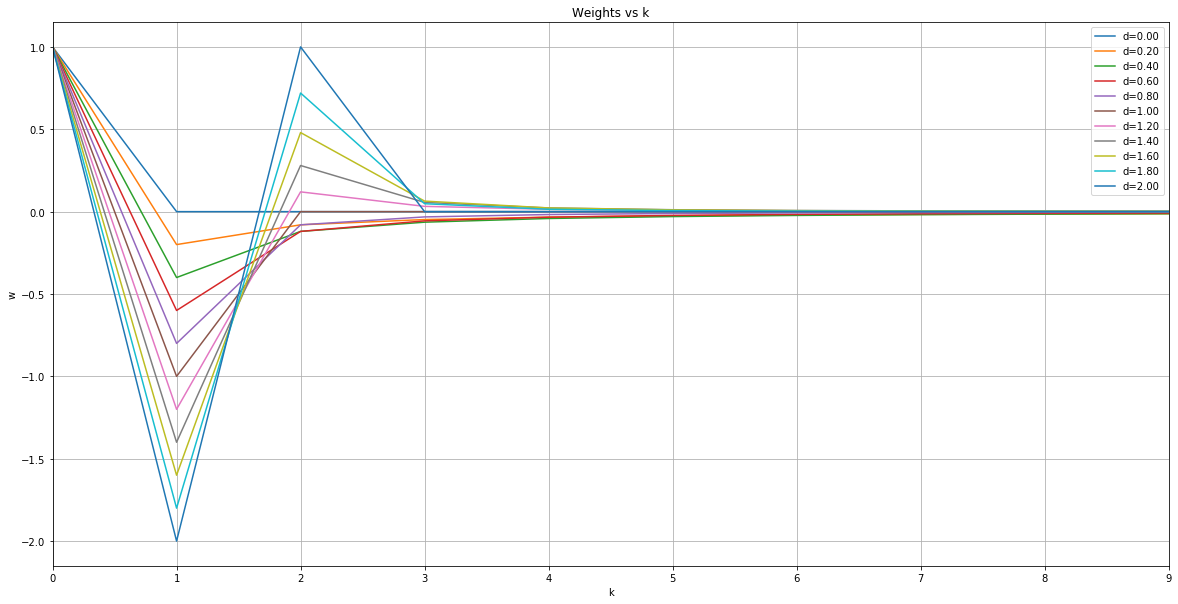
\includegraphics[width=\textwidth]{methods/images/weights_vs_k.png}
    \caption{Weight values vs. $k$ for different $d$ values.}
    \label{fig:w_k_vs_k}
\end{figure}

As it can be seen in figure \ref{fig:w_k_vs_k}, coefficients tend to zero as $k$
increases. It can also be proved the convergence of coefficients $w_k$. Let's
analyze the following when $k > d$ and $w_{k-1} \ne 0$:

\[|\frac{w_k}{w_{k-1}}| = |\frac{d-k+1}{k}| < 1 \]

what makes $|w_k| < |w_{k-1}|$ leading to $\lim_{k \to \infty} w_k = 0$.

When implementing fractional differentiation on a real time series, one has two
options:

\begin{enumerate}
  \item Adjust the length of $w_k$ vector by weight loss with a certain
        threshold.
  \item Work with a fixed number of coefficients.
\end{enumerate}

Option 1 requires the operation to compute the size of $w_k$ vector to account
for weight loss given a certain threshold. Weight loss cam be computed:

\begin{equation}
  \lambda_l = \frac{\sum_{j=T-l}^{T}|w_j|}{\sum_{i=0}^{T-1}|w_i|}
\end{equation}

where:

\begin{itemize}
  \item $T$ is the length of the time series,
  \item $l$ is the index of the sample from the end where the fractional
        differentiation occurs.
  \item $\lambda_l$ the weight loss at $l$ index
\end{itemize}

One should discard all samples whose $\lambda_l < \tau$ and $\tau$ is the
threshold. As $d \to 0$, the energy of the weights decreases leading to more
weight loss and more discarded samples.

Option 2 comes with the simplicity of having always the same vector of
coefficients $w_k$ such that $|w_k| > \tau$ and $\tau$ is a user defined
threshold. It comes with the advantage of having no drift as option 1 and just
needs to drop $l$ samples at the beginning, being $l$ the value of $l$ that
makes $w_k$ less or equal to $\tau$. In this thesis, option 2 is used.

So far, how to compute the weights vector was explained. Now, we just need to
address the value of $d$. $X_t$ might be stationary already which leads to
$d^* = 0$ with $d^*$ the value of $d$ that preserves most memory making the 
time series stationary. When $X_t$ has a \emph{unit root} (see chapter 15 of \cite{time_series_analysis}),
$0 \le d^* \leq 1$. And when $X_t$ exhibits an explosive (bubble) behavior,
$d^* > 1$. Unit roots can be tested with Dickey Fuller hypothesis test
(see chapter 17 of \cite{time_series_analysis}). The null hypothesis of the test claims the series has a unit root.
After determining a certain confidence level one can derive an \emph{optimum}
$d^*$ by:

\begin{enumerate}
  \item Define a vector of $d$ values in range of 0 to 1.
  \item For each value of $d$:
  \begin{enumerate}
    \item Fractionally differentiate $X_t$ with $d$ given a certain amount of
          weights. Obtain $X_t^d$.
    \item Compute the Dickey Fuller statistic, ADF, for $X_t^d$.
    \item Compute the p-value of the test.
  \end{enumerate}
  \item Choose $d^*$ that yields the maximum p-value between all p-values that
        are less or equal to the confidence level.
\end{enumerate}

This process has two flaws:

\begin{itemize}
  \item It is computationally time complex. Each time we apply the fractional
        differentiation, we are processing a $O(n^2)$ algorithm. Computing the
        ADF of the differentiated series requires a differentiation and model
        estimation which yields at least another $O(n^2)$ process. Finally, we
        iterate through a vector of $d$ adding another dimension.
  \item \emph{Optimum} $d$ is subject to the granularity of the $d$ vector of
        samples. The smaller the step, the more information one could preserve
        in the final time series, but the more iterations are required which
        impacts directly in the aforementioned item.
\end{itemize}

Regardless, all features that expose non-stationary characteristics could be
transformed and stabilized while preserving memory.
\subsubsection{Primary model}
\label{sec:methods_pipeline_primary_model}

The primary model consists of computing two moving average signals with
different time windows. The longer the time window, the more samples are
averaged and consequently the slower it varies with price variations. Having two
signals, one \emph{fast} and one \emph{slow} provides information of how short
and long term price movement vary one with respect to other. In particular, the
strategy takes advantage of the crossing points of both signals. When the fast
signal crosses above the slow signal, a buy event is generated. When the slow
signal crosses above the fast signal, a sell event is generated.

Note that from a daily sampled, positive and real signal as the bitcoin close
price in USD is, we obtain another two daily sampled, positive and real signals
(fast and slow). The latter two signals generate when they cross the events of
the primary model. These events are not equally spaced anymore, and the series
is categorical, its values are $\{1, -1\}$ which represent $\{buy, sell\}$
respectively. See figure \ref{fig:buy_and_sell_labels} to show these events over
the bitcoin price series.

\begin{figure}[H]
    \centering
    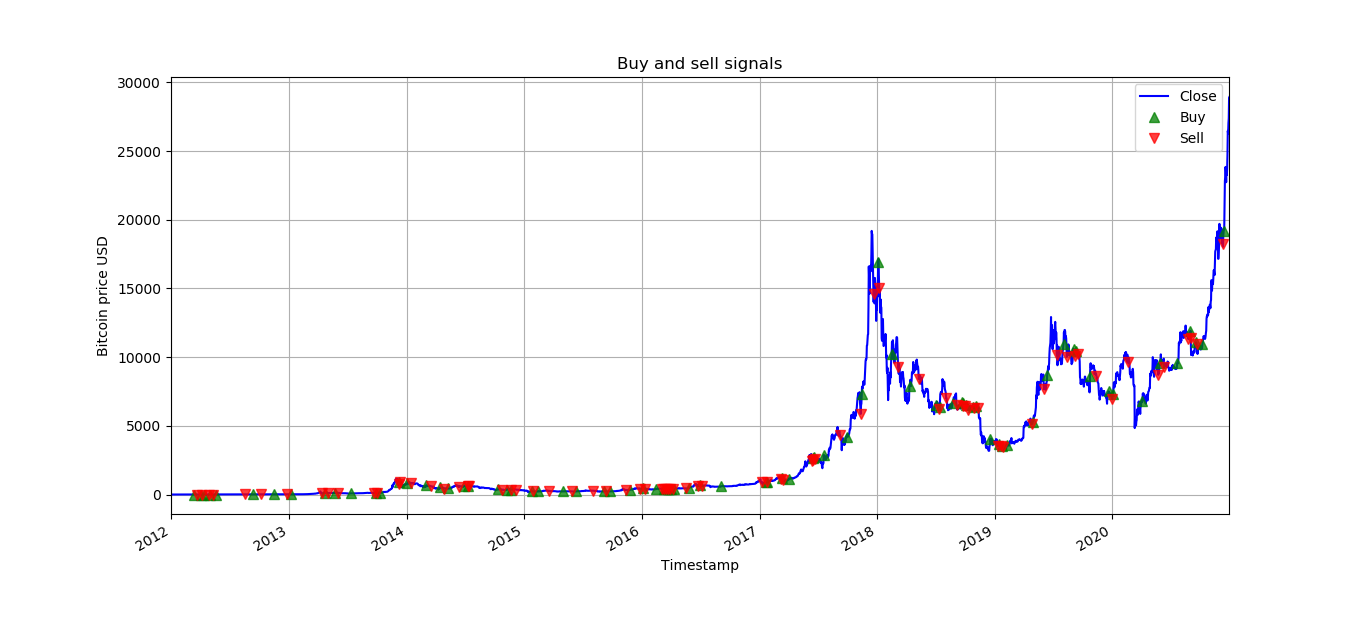
\includegraphics[width=\textwidth]{methods/images/buy_and_sell_labels.png}
    \caption{Buy and sell signals over the price series.}
    \label{fig:buy_and_sell_labels}
\end{figure}

The process of obtaining the signal with the bets is called \emph{labeling}
because it generates a series of \emph{labels} that determine a concrete action:
buy or sell the position. Next, \emph{metalabeling} process comes. It consists
in providing a probability to each \emph{label} which will be used to size the
bet. To assess whether the \emph{label} is correct or not, the triple barrier
method is used:

\begin{enumerate}
  \item Define a profit taking and stop loss rate for which a buy and sell
        signals will be considered valid. For a given price and time, a new
        greater value and lesser value are defined based on both rates before.
  \item Define a time constant $h$ (expressed as a positive and integer multiple
        of the sampling rate, i.e. number of days) that determines for each
        label, a new time stamp ahead.
  \item Determine whether the price signal hits the greater price or the lesser
        price before reaching the time stamp ahead of $h$ periods from the
        label's event. When:
  \begin{itemize}
    \item A $1$-valued label gets a cross with the greater price barrier, the
          metalabel is $1$ to indicate a positive label.
    \item A $-1$-valued label gets a cross with the lesser price barrier, the
          metalabel is $1$ to indicate a positive label.
    \item A $1$-valued label gets a cross with the lesser price barrier, the
          metalabel is $0$ to indicate a positive label.
    \item A $-1$-valued label gets a cross with the greater price barrier, the
          metalabel is $0$ to indicate a positive label.
    \item When both $1$ and $-1$ valued labels do not get a corresponding cross 
          with any of the price barriers, the return sign between the price at
          $h$ sample periods ahead of label's time stamp and the label's price
          is used. If the sign of the return and the label match, the metalabel
          is $1$, otherwise it is $0$.
  \end{itemize}
\end{enumerate}

Labels and metalabels are fundamental series to build the secondary model. The
secondary model is a classifier that is trained with metalabels. The predicted
probability will help to size the bet on each label. In mathematical terms:
$Metalabels = f_{(Labels, ...)}$ where $f$ represents the secondary model.
\subsubsection{Secondary model}
\label{sec:methods_pipeline_secondary_model}

The metalabelling process allows to algorithmically determine the positiveness
of the labels. Note that metalabels should not be included as input features
of the model because they belong to the future of the label and one model doing
that will not be plausible to implement on a real time system.
Initially, all features in the feature engineering section \ref{sec:methods_features}
will be used to build this model.

This research project will use bagging trees. In chapter 6 of \cite{lopez_de_prado}
there is a discussion about ensemble models and three are compared: bagging
trees, random forests and boosting. Boosting is generally superior in terms of
bias and variance results with respect to the others but it comes with, in my
opinion, an important penalty: the training process should be done sequentially whereas
bagging can be parallelized. The author is explicit about the other positive and
negative aspects such as tendency to over-fitting or under-fitting, by stating
that those claims are relative to how careful the researcher is when developing 
the training pipeline and curating data.

The focus of this research is not to get into the details of one machine
learning model or the other, but to explain the most relevant characteristics of
the one to be used and how its characteristics are used in favor of the research
problem at hand. Bagging ensembles rely on multiple, $B$, decision (or
regression but in this case we need decision) trees whose outcome is averaged 
to reduce the high variance of each tree. Decision trees tend to be deep, in
favor of bias reduction, but each tree variance is high. Increasing the number
of $B$ trees does not imply an immediate shift towards over-fitting what makes
it an appropriate hyperparameter to adjust in favor of variance reduction. See
section 8.2.1 of \cite{intro_to_statistical_learning} for a better
description of how bagging ensembles work.

Provided that only one dataset is available, a bootstrap sample method is used.
Bootstrapping consists of sampling the base dataset with replacement to generate
new datasets that will be used to train each decision trees. Each new dataset is
expected to be biased and the variance between datasets will be diminished when
averaging, or bagging, the results of the trees. Bootstrapping can also be done
with the features of the dataset. See section 5.2 of \cite{intro_to_statistical_learning}
for a concise but comprehensive description to bootstrapping.

The general bootstrapping method for samples assumes that all samples are IID.
This is not our case when using the triple barrier method.
Note that some samples might co-occur when time windows expand from the label
timestamp to $h$ sample periods ahead. In high volatility events, or with high
values of $h$, we should expect events, or labels, to happen while another one
is being evaluated. Weighing these labels with respect to unique and without any
overlap events is important to get the most out of the bootstrapping sampling
procedure. Following Lopez de Prado's analysis, concurrent labels are defined as
those that share at least one return attribution in the triple barrier method. 
Let the concurrency $c_t$ at time $t$ be defined as:

\[c_t = \sum_{i=1}^I l_{t,i}\]

Where $l_{t,i}$ is the i-th label value that occurs at $t$ and $I$ is the number of
label which co-occur at $t$. Labels start at a certain time $t$ but span a
number of sampling periods that could be $h$ or the time difference with respect
to one of the horizontal (price) barriers crossing events. Consequently, a label
will contribute to at least two different and consecutive timestamps and up to
$h$ consecutive timestamps.

Let the uniqueness of a label $i$ at time $t$ be defined as:

\[u_{t,i} = \frac{l_{t_i}}{c_t}\]

And the average uniqueness will be defined as the averaged uniqueness over the
label's lifespan:

\[\bar{u}_{t,i} = \frac{\sum_{t=1}^{T} u_{t,i}}{\sum_{t=1}^{T} l_{t,i}}\]

Label's average uniqueness allows a smarter bootstrap sampling method because it
can be used to prioritize events with higher uniqueness over the ones with less
uniqueness because the sole fact that they are weird in the dataset.

Lopez de Prado proposes a change to the above uniqueness sample weight. He
introduces the bet return also to account for an average of all the bets
simultaneously running. To do so, a new weight $w_i$ for label $i$ is proposed:

\[ \tilde{w}_i =\big| \sum_{t=t_{i,0}}^{t_{i,1}} \frac{r_{t-1,t}}{c_t} \big|\]

\[ w_i = \frac{\tilde{w}_i I}{\sum_{j=1}^{I} \tilde{w}_j}\]

Moving from $\tilde{w}_i$ to $w_i$ involves a scale factor to assure:
$\sum_{i=1}^{I} w_j = I$. When training the model, the training set / fold (when
using cross validation) will incorporate the weight with combined return and
uniqueness attribution to differentiate rare as well as rare high-return events
from the other concurrent and low-return events. Lopez de Prado also proposes a
sequential bootstrap method which updates the probability of each sample in the 
series every time a row is drawn. This process yields train sets closer to IID
but this is not part of this research pipeline.
\subsubsection{Training}
\label{sec:methods_pipeline_training}

The training stage involves tweaking both the primary model and the secondary
model. The primary model has the following hyperparameters:

\begin{itemize}
  \item Fast window period: the number of periods to average the price signal
        for the fast moving average signal.
  \item Slow window period: the number of periods to average the price signal
        for the slow moving average signal.
  \item Stop loss ratio: the price ratio when a label occurs that will determine
        the lower price barrier to determine the triple-barrier frontier.
  \item Profit taking ratio: the price ratio when a label occurs that will
        determine the higher price barrier to determine the triple-barrier
        frontier.
  \item Volatility time window: when applying the triple barrier method, a
        volatility series is computed out of daily returns. Volatility series is
        the result of an exponentially weighted moving average which takes the
        time window long samples and computes the standard deviation of it. This 
        series is used together with the minimum return.
  \item Minimum return: the primary model generates labels which involve really
        low returns and can be considered noisy samples. This threshold works 
        as a filter to discard these labels before they become part of the
        primary model output.
\end{itemize}

On the other hand, we have the secondary model which is a classifier. This
classifier will be used to determine the size of the bets. In section \ref{sec:methods_pipeline_secondary_model}
it was mentioned that it will be a Bagging classifier whose parameters are:

\begin{itemize}
  \item Number of estimators: the number of trees to train ($B$)
        and then take the majority vote for each new estimation.
  \item Number of samples per estimator: the fraction of samples in the dataset
        to sample with or without bootstrap. This value is set to the average
        uniqueness of all labels.
  \item Use bootstrap: whether to use or not bootstrap sampling. This value is
        set to true. On top of it, when fitting, the particular label uniqueness
        is used.
  \item Maximum of features to use: out of all predictors, how many features per
        estimator to use. No bootstrap is used at the predictor level, just a
        sampling. 
\end{itemize}

Unless explicitly mentioned, all hyperparameters are optimized. For the primary model,
the following criteria is used:

\begin{itemize}
  \item For certain combinations of hyperparameters, there might not be
        enough labels and metalabels to train the secondary model training process.
        Also, the primary model might output a too imbalanced set of labels and
        metalabels which end up causing trouble when training because of lack of
        one class of metalabel. The generated model out of that hyperparameters are
        discarded. 
  \item For certain combinations of hyperparameters, there might be very little
        amount of samples. These combinations are discarded.
  \item Using a quite simple secondary model of the same nature but without
        optimized hyperparameters, we choose the combination of primary model
        hyperparameters that yield better secondary performance.
\end{itemize}

Performance in the secondary model is evaluated with negative logarithmic loss.
Typically, classifiers use F1-score because they provide a good balance between
precision and recall (its the harmonic mean between both). In this case, we are
mostly interested in selecting models based on the predicted probabilities
because that is used to size bets.

Secondly, once the primary model hyperparameters have been selected, a full
model optimization for the secondary model is done. Again, negative logarithmic loss is
used to determine the best model. Following Lopez de Prado recommendations in
chapter 7 of \cite{lopez_de_prado}, purged $K$-fold cross validation with embargo
is used to train the secondary model.

\paragraph{Purge:} when the classification output at time $t$, i.e. metalabel,
depends on the value of the predictor(s) at two or more sample values, we have
an inter-time dependency of the output with several of the predictors that might
lead to leakage if they are not properly purged. The purge strategy consists on
removing the predictor and classification outputs that are concurrent in
adjacent training and test folds. There are three situations that would make two
labels concurrent:

\begin{itemize}
  \item Label $i$ starts inside the triple barrier period of label $j$.
  \item Evaluation of metalabel $i$ ends inside the triple barrier period of
        label $j$.
  \item Evaluation of label $j$ starts and ends inside the triple barrier period
        of label $i$.
\end{itemize}

In addition to this concurrency effect, there is another effect that produces
information leakage between train-test splits. Suppose a label that is assigned
to a test fold and it is generated from data that is spread in multiple
labels both in train and test folds even though there is no label concurrency
involved, there will be leakage. In this case purge is also required to mitigate
leakage.


\paragraph{Embargo:} when there is no clear time span that is required to ban
from the adjacent training and test folds to avoid leakage due to the nature of
the classification output generation process, the embargo technique can be used.
It consist of removing a percentage of samples in the train fold that are right
after the test fold beginning. Note that there is no need to remove samples from
the end of the test fold when it is adjacent to another training fold because
those samples will simply not contribute to train the model for the first set
of labels. The percentage is usually low, e.g. 1\%, and provides enough data
pruning to run the training stage without noticeable leakage.

\subsubsection{Feature importance}
\label{sec:methods_pipeline_feature_importance}

Lopez de Prado's eloquent words in section 8.2 of \cite{lopez_de_prado} are very
appropriate to illustrate what this section is about.

\say{Hunters do not blindly eat everything their smart dogs retrieve for them, do they?}

As a financial machine learning researcher once we are satisfied
with the performance of a machine learning model it is advised to understand
which, how and when features contribute to improve the performance of the model.
The author focuses on the \emph{importance} of the features with and without
substitution effects. In this research pipeline, only a method to consider
substitution effects is implemented.

The method is called Mean Decrease Accuracy and it uses model's estimation
accuracy as guiding principle. Description of the method follows:

\begin{itemize}
  \item Let $X$ of be the feature matrix and let $Y$ be the output vector.
  \item Let $X_1, X_2, X_3, ..., X_m$ be the columns of $X$.
  \item Fit via the desired training process $m + 1$ models and measure their
        accuracy. One model will be fitted with $X$ as is. And the other $m$
        models will be fitted with one randomly permutated column $X_i$.
  \item For each of the aforementioned $m$ models, compute the relative loss in
        accuracy with respect to the base without permutation model. 
\end{itemize}

This method allows to create a rank in which once can inspect the relative loss
of performance measured in accuracy, but it could also be F1-score or
negative log-loss when working with classifiers. Having a high value means
that the predictive importance of the feature is relevant. Even though this method
is flexible and adaptable to multiple types of models as it is based on out of
sample performance, it comes with some important drawbacks:

\begin{itemize}
  \item It is relatively slow because it requires the training of $m + 1$ models and
        the evaluation of their performance. When this is done with purged $K$-fold cross
        validation with embargo\emph{ed} datasets, it will definitely take time.
  \item It is susceptible to \emph{substitution effects}. The effect can be described with two
        or more features that are highly correlated. The performance loss will be similar so
        a researcher might decide to remove them but with that the overall predictive 
        capacity diminishes more than just keeping one of the features in the set
        under study.
  \item A possible result is that all features are detrimental or unimportant
        for the model what is somewhat hard to interpret.
\end{itemize}

Feature orthogonalization could help to reduce the substitution effect. Two
procedures are proposed. First, a direct application of Frisch–Waugh–Lovell theorem
analysis can be used. Each feature is analyzed individually via a linear
regression and residues are inspected to derive relative importance. See
chapters 2 and 3 of \cite{econometric_theory_and_methods} for an in depth description
of the theorem and applications. Secondly, Principal Component Analysis, i.e. PCA,
as suggested in section 8.4.2 of \cite{lopez_de_prado} can also be used to
determine the set of features whose eigenvalues in the orthogonalized space are
greater. Alternatively, the feature space could also be reduced in favor of
faster convergence of the machine learning models under use.

Once all features are ranked, the researcher is required to select which
features to drop and which ones to keep. The final set of features will be used
to build a new model. Heuristic rules are used to drop features but as mentioned
before researchers should be aware of the substitution effect. In this research
project, the applied rule applied consists in computing the mean loss of
negative log-loss and keep those features that produce higher than the mean loss
in performance.

Furthermore, researchers often face the requirement of explaining the economic
mechanism that generates the excess return of the strategy with respect to a
benchmark. Understanding which features contribute more to predict with increased
confidence labels is reasonably simpler when extra unimportant features are
removed. This stage of the process together with feature engineering are very
important to understand how the model behaves.
\subsubsection{Bet sizing}
\label{sec:methods_pipeline_bet_sizing}

Labels and metalabels will be used together with other features to train a secondary
model whose output estimated probability for each new label will be used to size
the bet for that event. One way to do this is to scale the predicted probability,
by the budget total and get value in currency for the bet. However, if we did so,
there would not be any awareness about other concurrent bets, so we might misuse
the available budget to run other concurrent bets. Lopez de Prado in chapter 10
of \cite{lopez_de_prado} proposes the following:

\begin{enumerate}
  \item Let $p_{(x)}$ be the probability of label $x$ that takes the one of the
        values in $[-1, 1]$.
  \item Run a statistical test where $H_{0}: p_{(x=1)} = 0.5$ with the statistic
        $z = \frac{p_{(x=1)} - 0.5}{\sqrt{0.5(1-0.5)}} = \frac{p_{(x=1)} - 0.5}{0.5}$
  \item Let the bet size $m$ be: $m = 2 \Phi_{(z)} - 1$ where $\Phi_{(z)}$ is
        the cumulative distribution function of the standard normal
        distribution. $m \in [-1; 1]$
\end{enumerate}

Once we have a vector of $m$ values, which has a one to one relationship with
each label $x$, we can average the bet with those concurrent triple barrier
windows as the come in the pipeline. Averaging does not change the bet size
for open windows, but changes the size for new bets that overlap with open
windows.

Finally, a portfolio manager might also consider bet size discretization by
means of setting an integer number of equally sized budget partitions. The
discretized value of the bet after the average is $m^* = round\Bigg( \frac{m}{d} \Bigg) d$
where $d = \frac{1}{Number of partitions}$. And the only remaining step when
running the strategy is to scale the budget by $m^*$ to have the final bet size
in currency. The goal of this step is to reduce jitter which causes overtrading.
Typical number of partitions are below ten.

\subsubsection{Back testing}
\label{sec:methods_pipeline_backtesting}

This section focuses on explaining how this exercise would be 
carried out, the differences with respect to the implemented
back testing strategy and how benchmarking metrics are affected.
Also, metrics are explained.

\paragraph{Strategy} The strategy will start at certain date with an
initial budget of \$1,000,000 dollars (USD) to spend as both 
the primary and secondary model dictate. Every day, new features are gathered
and processed together with the historical data. Feed the selected set of
columns that conform the secondary model and the primary model determines
whether a new label and metalabel should be created and then the secondary model
proposes a probability for that metalabel. The bet sizing transformation will
scale and determine a dollar level for the bet. Depending on the position the
primary model proposes and the bet size, the following steps are conducted:

\begin{itemize}
  \item When placing a long position and the bet size is not zero:
  \begin{enumerate}
    \item Bet size dollars are taken from the portfolio at time $t$.
    \item Bet size dollars are used to buy bitcoins. The BTC/USD
          rate is the price at the moment where the order takes place. From the
          bet size dollars, the exchange buy fee is discounted from the bet
          size.
    \item We hold the long position until one of the three barriers
          of the triple barrier boundaries is crossed by the price 
          path. The primary model defined by hyperparameter 
          optimization a value for the stop loss, the profit taking and the
          holding period for the triple barrier, those values are computed based
          on the bitcoin price level at $t$.
    \item When the price series crosses any of the barriers, the 
          long position is closed and a sell fee is paid to the exchange.
    \item At this point, the value of the portfolio would be damaged 
          because of the buy and sell fees and benefited from the
          expected rise in bitcoin valuation measured in dollars. It
          is worth pointing out that the bet could end up having a
          net negative effect on the value of the portfolio.
  \end{enumerate}
  \item When placing a short position and the bet size is not zero:
  \begin{enumerate}
    \item Bet size dollars are taken from the portfolio at time $t$.
    \item A loan in bitcoins is requested. The bet size amount is
          used to pay the loan and pay the collateral amount.
    \item Those bitcoins are sold, consequently we get their 
          dollar valuation minus the sell fee of the exchange.
    \item We hold the short position until one of the three barriers
          of the triple barrier boundaries is crossed by the prices path. The
          primary model defined by hyperparameter optimization a value for the
          stop loss, the profit taking and the holding period for the triple
          barrier, those values are computed based on the bitcoin price level
          at $t$.
    \item When the price series crosses any of the barriers, the 
          short position is closed. In this case, bitcoins are bought
          to complement the collateral amount and return the loan interest.
    \item At this point, the value of the portfolio would be damaged 
          because of the buy and sell fees and the loan interest. However, it
          would benefit from the price drop and the short position.
  \end{enumerate}
\end{itemize}

The aforementioned procedures are iterated over the lifespan of the strategy and
must be monitored as any other strategy. Also, it is worth mentioning the risks
involved in the operation:

\begin{itemize}
  \item If the price path rapidly crosses the upper price level barrier before a 
        new price sample comes in (when evaluating sell orders) or it crosses the lower price
        level barrier before a new price sample comes in (when evaluating buy orders), there is
        an extra cost incurred due to a lack of live price monitor. It can be
        mitigated by having such monitor and an automatic order placing system.
  \item If having automatic control to place orders, the price path can simply
        not be enough to pay off the fees, even though the net return the price only is positive (accounting the transaction cost reduces the net profit from the trade).
\end{itemize}  

The portfolio manager will also have to consider how the collateral valuation
varies with time. Note that many bets time windows can overlap which
could cause budget starvation if highly confident bets co-occur.
Consequently, the collateral valuation will be affected by all short and
concurrent positions and with the price variations of the asset under management
and will reduce the effective return of each bet because of the compromised
savings to pay back the loan. However, it is worth mentioning that in case of a
an undesired rise in prices, the collateral will help to reduce the impact.

In this research project, we make the following assumptions:

\begin{itemize}
  \item Buy and sell exchange fees might vary over time. For simplicity, they
        are kept the same for the entire back testing period.
  \item Loan interests vary their every day. For
        simplicity, they are kept the same for the entire back testing period.
  \item Collateral budgets are not considered. Instead, a penalty to the loan
        interest is added.
  \item Because of considering the collateral budget as an extra interest, the
        value of the portfolio does not benefit from intra bet windows
        bitcoin price variation.
  \item Orders might not get processed during high price corrections. Those
        scenarios are not contemplated either.
\end{itemize}

In general, all of these simplifications will imply higher performance which is
perceived as excess returns.

As a reference, table \ref{table:benchmark_fees} contains the fees and rates involved in the strategy.

\begin{table}[H]
  \centering
  \begin{tabular}{| c | c |} 
    \hline
    \multicolumn{2}{|c|}{Fees} \\
    \hline
    Fee & Value \\
    \hline
    Buy & 0.10\% \\
    \hline
    Sell & 0.10\% \\
    \hline
    Loan interest & 5\% \\
    \hline
  \end{tabular}
  \caption{Financial metrics benchmark.}
  \label{table:benchmark_fees}
\end{table}

Buy and sell fees were take from Binance \cite{binance_fees} and loans from 
DefiRate \cite{defi_rate_loans} where an average has been done and a 1\% extra
has been added.

\paragraph{Benchmark} A base strategy is required to provide a reference and
compare against the output strategy of this research. Buying bitcoins the first
day and holding them until the last day of the testing period will be used. This
is an obvious choice because machine learning enhanced momentum is used over this
asset and would set a valid benchmark for this strategy.

\paragraph{Metrics} The secondary model will be measured with two metrics which
are appropriate for classification problems. The F1-score as a measure of the 
accuracy of the classifier. Then, to measure classifier performance, negative
logarithmic loss will be used to assess how well predicted probabilities adjust
to validation labels.

The strategy will be evaluated by the following metrics which also cover different
types:

\begin{itemize}
  \item Performance metrics:
  \begin{itemize}
    \item Win loss ratio: the ratio between positive returns and negative returns.
          The bigger the ratio, the better.
    \item Win rate: the ratio of positive returns over the total number of
          returns. The bigger the ration, the better.
    \item Average return: the arithmetic average of all returns. It is an estimate of the
          true mean return.
  \end{itemize}
  \item Efficiency metrics:
  \begin{itemize}
    \item Sharpe Ratio: measures the ratio between the average sample returns minus a risk free interest rate\footnotemark, and
          the sample standard deviation. It provides an estimate of the true
          Sharpe Ratio.
    \item Probabilistic Sharpe Ratio: expresses the probability that estimated
          Sharpe Ratio (see above) is higher than a benchmark Sharpe Ratio. See
          below for an in detail discussion.
    \item Sortino ratio: it is similar to the Sharpe Ratio in the sense that provides a
          a risk adjusted return ratio but it penalizes negative returns. It is
          generally a better choice to compare skewed return distributions. As the
          Sortino ratio increases the strategy becomes more appealing for a given
          benchmark target return. See \cite{sortino_a_sharper_ratio} for an
          analysis and explanation of the ratio.
  \end{itemize}
  \item Implementation shortfall metrics:
  \begin{itemize}
    \item Return on execution costs: ratio between the sum of all net returns
          (after operation costs) and the sum of all transaction costs. The bigger
          the ratio is, the more confident a portfolio manager will be about the
          strategy. Transaction costs cannot be known beforehand and high values
          cover for increased costs at execution time.
  \end{itemize}
  \item General metrics:
  \begin{itemize}
    \item Correlation to underlying: the correlation between the strategy and the
          underlying investment universe. As it gets closer to one or minus one,
          the closer it is to the benchmark strategy.
    \item Volatility: the standard deviation of the returns. It is an estimate of
          the true return standard deviation.
  \end{itemize}
\end{itemize} 

\footnotetext{Using US treasury yield annual curves \cite{treasury_yield}, one can observe that risk free interest rates vary from 0.05\% to 2.74\%. It means that the daily risk free interest rate varies from $2.73 x 10^{-6}$ to $7.4 x 10^{-5}$. It was simply considered zero.}

Moreover, it is important to discuss the Probabilistic Sharpe Ratio. It was
introduced in \cite{sharpe_paper} which compliments the information of the
estimated Sharpe Ratio which is usually provided in financial benchmarks.
For both strategies, the benchmark and the strategy under test, the true mean
and standard deviation of the Sharpe Ratio is and will remain unknown. Back
testing over past or generated data will only provide an estimate that adjusts
to the sample consequently, the Probabilistic Sharpe Ratio helps to understand
which is the probability that the estimated Sharpe Ratio is bigger than a set of
target ratios.

Furthermore, the estimate of the Sharpe Ratio mean comes from non IID return samples. Hence, Bailey and 
Lopez de Prado introduced an adjustment by skewness and kurtosis to the standard
error used in the statistical test. Then, it is appropriate to use a series of
target Sharpe Ratio to compare with and determine the probability that the
estimated Sharpe Ratio of our strategy is bigger for proposed target ratios. As a
reference, the Sharpe Ratio and the Probabilistic Sharpe Ratio formulas are copied
below.

\[\hat{SR} = \frac{\hat{r}}{s_{r}}\]

Where:

\begin{itemize}
  \item $\hat{SR}$ is the estimated Sharpe Ratio.
  \item $\hat{r}$ is the average return.
  \item $\hat{s_{r}}$ is the sample standard deviation of the returns.
\end{itemize}

\begin{equation}
  \label{eqn:prob_sharpe_ratio}
  \hat{PSR}_{(SR^*)} = \Phi \Bigg( \frac{(\hat{SR} - SR^*) \sqrt{N-1}}{\sqrt{1 - \hat{\gamma_3}\hat{SR} + \frac{\hat{\gamma_4} - 1}{4}\hat{SR}^2}} \Bigg)
\end{equation}

Where:

\begin{itemize}
  \item $\hat{PSR}_{(SR^*)}$ is the Probabilistic Sharpe Ratio for the reference
        Sharpe Ratio $SR^*$.
  \item $N$ is the number of returns in the sample to compute the index.
  \item $\hat{\gamma_3}$ is the sample return skewness.
  \item $\hat{\gamma_4}$ is the sample return kurtosis.
  \item $\Phi()$ is the cumulative distribution function of the standard Normal
        distribution.
\end{itemize}

\paragraph{Taxation} A potentially relevant “transaction cost” relates to taxes.
For example, in the US, and depending on the tax bracket, federal taxes for
short-term capital gains are taxed at up to 37\%\footnotemark . Capital gain taxes would
disfavor active trading on a highly volatile asset in our results.

\footnotetext{See \href{https://www.irs.gov/pub/irs-drop/rp-19-44.pdf}{26 CFR 601.602: Tax forms and instructions.}}
% @}

\newpage
% @}

% @{ Results
\subsection{Features}
\label{sec:methods_features}


In this section, all the features of the model are introduced. We will present
univariate and bivariate analysis of the features as well as different
techniques to transform them, in particular fractional differentiation.

When working with inference models, features should be stationary. Common
procedures to features like prices involve integer differentiation to end up
working with price returns instead. The latter would remove entirely the price
series memory which is required by the model to effectively predict the output.
Other methods involve applying power transformations such as logarithms, square
roots or box-cox transformations. We are not interested in those for price series.
They will drastically affect scales and might collapse movements around the trend
while preserving the trend.

In \cite{frac_diff_paper} the fractional differentiation method was introduced,
and Lopez de Prado takes the method and explains the model in chapter 5 of
\cite{lopez_de_prado}. I will present the mathematical model and explain the
algorithm in what follows.

Let $B$ be a backshift operator, i.e. delay operator, to be applied to a matrix 
of real valued features $X_{t}$ such that $B^k X_t = X_{t-k}$. Also, we can 
express the positive integer powers of a binomial as $(x+y)^n = \sum_{k=0}^n {n \choose k} x^k y^{n-k}$.
When considering real valued exponents, combinatorial number ${n \choose k}$
becomes (after substitution of $n$ an integer by $d$ a real number) ${d \choose k} = \frac{d (d-1) ... (d-k+1)}{k!}$
which coincides with the integer formula. Thus,

\begin{equation}
  \label{eqn:binomial_expantion_frac_power}
  (x+y)^d = \sum_{k=0}^{\infty} {d \choose k} x^k y^{d-k}
\end{equation}

Equation \ref{eqn:binomial_expantion_frac_power} presents an infinite series, a
key difference with respect to the integer counterpart. If we replace $x$ by $1$
and $y$ by $-B$, the backshift operator, one can write from \ref{eqn:binomial_expantion_frac_power}:

\[(1-B)^d = \sum_{k=0}^{\infty} {d \choose k} (-B)^k \]

\[(1-B)^d = \sum_{k=0}^{\infty} \frac{\prod_{i=0}^{k-1}(d-i)}{k!} (-B)^k \]

\begin{equation}
  \label{eqn:binomial_expantion_diff_operator}
  (1-B)^d = 1 - dB + \frac{d(d-1)}{2!}B^2 - \frac{d(d-1)(d-2)}{3!}B^3 + ...
\end{equation}

Equation \ref{eqn:binomial_expantion_diff_operator} presents the foundation of
the fractional differentiation method. If one could find the value of $d$ such
that a series $X$ gets differentiated and becomes stationary while preserving
as much memory as possible a later model would be able to exploit that memory to
predict the output. In particular, when the value of $d$ ends up being less than 1.
Equation \ref{eqn:binomial_expantion_diff_operator} also
presents a problem, it is a infinite series when $d$ is noninteger which makes
the operation to be non exact for the general case due to the impossibility of
applying infinite multiplications and sums. Lopez de Prado proposes a solution
for both issues.

A fractionally differentiated series $X$ can be expressed for a given $d$ as: 

\[ X_t^d = \sum_{k=0}^{\infty} w_k X_{t-k} \]

The vector $w$ of weights in the above equation follows:

\begin{equation}
  \label{eqn:ffd_weights}
	w = {1, -d, \frac{d(d-1)}{2!}, -\frac{d(d-1)(d-2)}{3!}, ..., (-1)^k \prod_{i=0}^{k-1} \frac{(d-i)}{k!}} 
\end{equation}

One can derive by inspection of equation \ref{eqn:ffd_weights} a generative and
recursive expression for each item in the series:

\begin{equation}
  \label{eqn:ffd_weights_generative}
  w_k = -w_{k-1} \frac{d-k+1}{k}
\end{equation}

Equation \ref{eqn:ffd_weights_generative} is easy to implement as a programming
function which is ideal for this application. It is also interesting to evaluate
the tendency of $w_k$ as $k$ tends to infinite, see figure \ref{fig:w_k_vs_k}.

\begin{figure}[!htb]
    \centering
    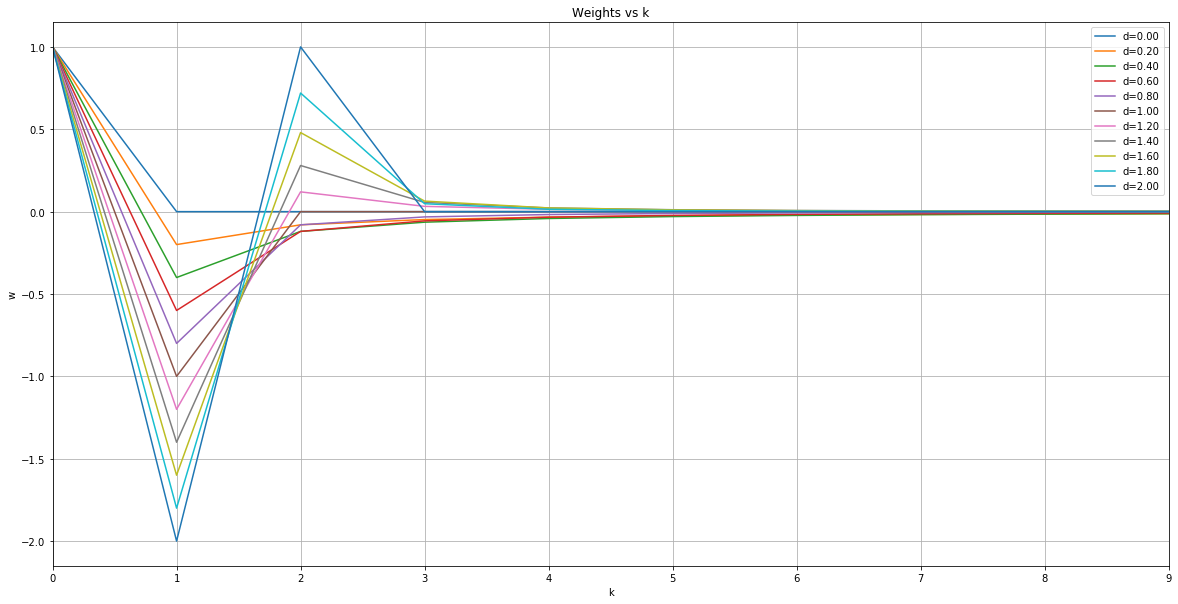
\includegraphics[width=\textwidth]{methods/images/weights_vs_k.png}
    \caption{Weight values vs. $k$ for different $d$ values.}
    \label{fig:w_k_vs_k}
\end{figure}

As it can be seen in figure \ref{fig:w_k_vs_k}, coefficients tend to zero as $k$
increases. It can also be proved the convergence of coefficients $w_k$. Let's
analyze the following when $k > d$ and $w_{k-1} \ne 0$:

\[|\frac{w_k}{w_{k-1}}| = |\frac{d-k+1}{k}| < 1 \]

what makes $|w_k| < |w_{k-1}|$ leading to $\lim_{k \to \infty} w_k = 0$.

When implementing fractional differentiation on a real time series, one has two
options:

\begin{enumerate}
  \item Adjust the length of $w_k$ vector by weight loss with a certain
        threshold.
  \item Work with a fixed number of coefficients.
\end{enumerate}

Option 1 requires the operation to compute the size of $w_k$ vector to account
for weight loss given a certain threshold. Weight loss cam be computed:

\begin{equation}
  \lambda_l = \frac{\sum_{j=T-l}^{T}|w_j|}{\sum_{i=0}^{T-1}|w_i|}
\end{equation}

where:

\begin{itemize}
  \item $T$ is the length of the time series,
  \item $l$ is the index of the sample from the end where the fractional
        differentiation occurs.
  \item $\lambda_l$ the weight loss at $l$ index
\end{itemize}

One should discard all samples whose $\lambda_l < \tau$ and $\tau$ is the
threshold. As $d \to 0$, the energy of the weights decreases leading to more
weight loss and more discarded samples.

Option 2 comes with the simplicity of having always the same vector of
coefficients $w_k$ such that $|w_k| > \tau$ and $\tau$ is a user defined
threshold. It comes with the advantage of having no drift as option 1 and just
needs to drop $l$ samples at the beginning, being $l$ the value of $l$ that
makes $w_k$ less or equal to $\tau$. In this thesis, option 2 is used.

So far, how to compute the weights vector was explained. Now, we just need to
address the value of $d$. $X_t$ might be stationary already which leads to
$d^* = 0$ with $d^*$ the value of $d$ that preserves most memory making the 
time series stationary. When $X_t$ has a \emph{unit root} (see chapter 15 of \cite{time_series_analysis}),
$0 \le d^* \leq 1$. And when $X_t$ exhibits an explosive (bubble) behavior,
$d^* > 1$. Unit roots can be tested with Dickey Fuller hypothesis test
(see chapter 17 of \cite{time_series_analysis}). The null hypothesis of the test claims the series has a unit root.
After determining a certain confidence level one can derive an \emph{optimum}
$d^*$ by:

\begin{enumerate}
  \item Define a vector of $d$ values in range of 0 to 1.
  \item For each value of $d$:
  \begin{enumerate}
    \item Fractionally differentiate $X_t$ with $d$ given a certain amount of
          weights. Obtain $X_t^d$.
    \item Compute the Dickey Fuller statistic, ADF, for $X_t^d$.
    \item Compute the p-value of the test.
  \end{enumerate}
  \item Choose $d^*$ that yields the maximum p-value between all p-values that
        are less or equal to the confidence level.
\end{enumerate}

This process has two flaws:

\begin{itemize}
  \item It is computationally time complex. Each time we apply the fractional
        differentiation, we are processing a $O(n^2)$ algorithm. Computing the
        ADF of the differentiated series requires a differentiation and model
        estimation which yields at least another $O(n^2)$ process. Finally, we
        iterate through a vector of $d$ adding another dimension.
  \item \emph{Optimum} $d$ is subject to the granularity of the $d$ vector of
        samples. The smaller the step, the more information one could preserve
        in the final time series, but the more iterations are required which
        impacts directly in the aforementioned item.
\end{itemize}

Regardless, all features that expose non-stationary characteristics could be
transformed and stabilized while preserving memory.
\subsection{Model results}
\label{sec:model_results}

\paragraph{Training} The strategy has been optimized using a random search in
the hyperparameter space as commented in section \ref{sec:methods_pipeline_training}.
Primary model results are shown in table \ref{table:primary_model_hyperparameters},
and secondary model results are shown in table \ref{table:secondary_model_hyperparameters}.

\begin{table}[H]
  \centering
  \begin{tabular}{|c | c |} 
    \hline
    \multicolumn{2}{|c|}{Primary model} \\
    \hline
    Parameter & Value \\
    \hline
    Moving average fast window length & 5 \\
    \hline
    Moving average slow window length & 30 \\
    \hline
    Profit taking band                & 0.06 \\
    \hline
    Stop loss taking band             & 0.02 \\
    \hline
    Triple barrier window length      & 3 \\
    \hline
    Minimum return                    & 0.005 \\
    \hline
    Volatility window length          & 50 \\
    \hline 
  \end{tabular}
  \caption{Primary model hyperparameters.}
  \label{table:primary_model_hyperparameters}
\end{table}

\begin{table}[H]
  \centering
  \begin{tabular}{|c | c |} 
    \hline
    \multicolumn{2}{|c|}{Secondary model} \\
    \hline
    Parameter & Value \\
    \hline
    Number of estimators                & 720 \\
    \hline
    Maximum features ratio when bagging & 0.2936 \\
    \hline
    Average uniqueness                  & 0.9502 \\
    \hline
    Cross validation splits             & 6 \\
    \hline
    Embargo                             & 1\% \\
    \hline
  \end{tabular}
  \caption{Secondary model hyperparameters.}
  \label{table:secondary_model_hyperparameters}
\end{table}

\paragraph{Labels} The output of the primary model is summarized in table
\ref{table:labels_metalabel} where we also show the labels and metalabels count.
Also, in \ref{table:label_vs_metalabel} a contingency table between 
labels and metalabels is shown. We can see that even though labels are balanced,
there is a bias towards negative metalabels (i.e. do not take the bet) based on
the triple barrier parameters.

\begin{table}[H]
  \centering
  \begin{tabular}{| c | c |} 
    \hline
    \multicolumn{2}{|c|}{Labels}      \\
    \hline
    Value & Count                     \\
    \hline
    1 (buy signal) & 80               \\
    \hline
    -1 (sell signal) & 79             \\
    \hline
    \multicolumn{2}{|c|}{Metalabels}  \\
    \hline
    Value & Count                     \\
    \hline
    0 (unreliable label)     & 103    \\
    \hline
    1 (reliable label)       & 56     \\
    \hline
  \end{tabular}
  \caption{Primary model labels and metalabels.}
  \label{table:labels_metalabel}
\end{table}

\begin{table}[H]
  \centering
  \begin{tabular}{|c|c|c|}
    \hline
    Label     & \multirow{2}{*}{0} & \multirow{2}{*}{1} \\ \cline{1-1}
    Metalabel &                    &                    \\ \hline
    1         & 51                 & 29                 \\ \hline
    -1        & 52                 & 27                 \\ \hline
  \end{tabular}
  \caption{Contingency table between labels and metalabels.}
  \label{table:label_vs_metalabel}
\end{table}

\paragraph{Feature importance} Table \ref{table:feature_importance_results}
shows the mean loss in performance per feature after applying the method explained in
\ref{sec:methods_pipeline_feature_importance}. Note that only those features
with mean loss in performance above the mean loss are shown. See figure
\ref{fig:feat_importance} for an in detail mean loss of performance and standard
deviation per feature permutation.

It is interesting to point the groups of features that remained in the final model:

\begin{itemize}
  \item Price and volume features with fractional differentiation.
  \item SADF derived indices with different regression models (constant, linear and
        quadratic) and with one, two and three lag periods for the autocorrelation.
  \item Volatility and logarithmic returns.
  \item Market capitalization.
  \item Fees, transfer volume and days till halving. These are features related
        to the bitcoin ecosystem. 
\end{itemize}

However, none of the social features seemed to produce a high impact in the final
model.

\begin{table}[H]
  \centering
  \begin{tabular}{| c | c | c |} 
    \hline
    \multicolumn{3}{|c|}{Feature importance} \\
    \hline
    Feature                     & Mean perf. loss & Std. dev. of perf. loss\\ \hline
    CloseFFD                    & 0.039714        & 0.026393 \\ \hline
    HighFFD                     & 0.018739        & 0.019605 \\ \hline
    LowFFD                      & 0.002177        & 0.001215 \\ \hline
    OpenFFD                     & 0.006869        & 0.003897 \\ \hline
    Volume\_(BTC)-log            & 0.032430        & 0.015899 \\ \hline
    Volume\_(Currency)-log       & 0.020350        & 0.008696 \\ \hline
    bsadf\_ct\_1                  & 0.002128        & 0.002060 \\ \hline
    bsadf\_ctt\_1                 & 0.003910        & 0.003278 \\ \hline
    bsadf\_ctt\_2                 & 0.004907        & 0.004139 \\ \hline
    bsadf\_ctt\_3                 & 0.003264        & 0.004178 \\ \hline
    bsadf\_nt\_2                  & 0.003447        & 0.004077 \\ \hline
    daysTillHalving             & 0.003387        & 0.003194 \\ \hline
    fees-mean-log               & 0.004142        & 0.002743 \\ \hline
    log\_ret                     & 0.013930        & 0.006140 \\ \hline
    market-cap-log              & 0.002412        & 0.001501 \\ \hline
    transfer-volume-median-log  & 0.006073        & 0.006431 \\ \hline
    trgt                        & 0.003003        & 0.007776 \\ \hline
    vol\_15                      & 0.008678        & 0.003120 \\ \hline
    vol\_5                       & 0.020516        & 0.015831 \\ \hline
  \end{tabular}
  \caption{Feature performance loss of the secondary model. Only selected features are displayed.}
  \label{table:feature_importance_results}
\end{table}

\begin{figure}[H]
    \centering
    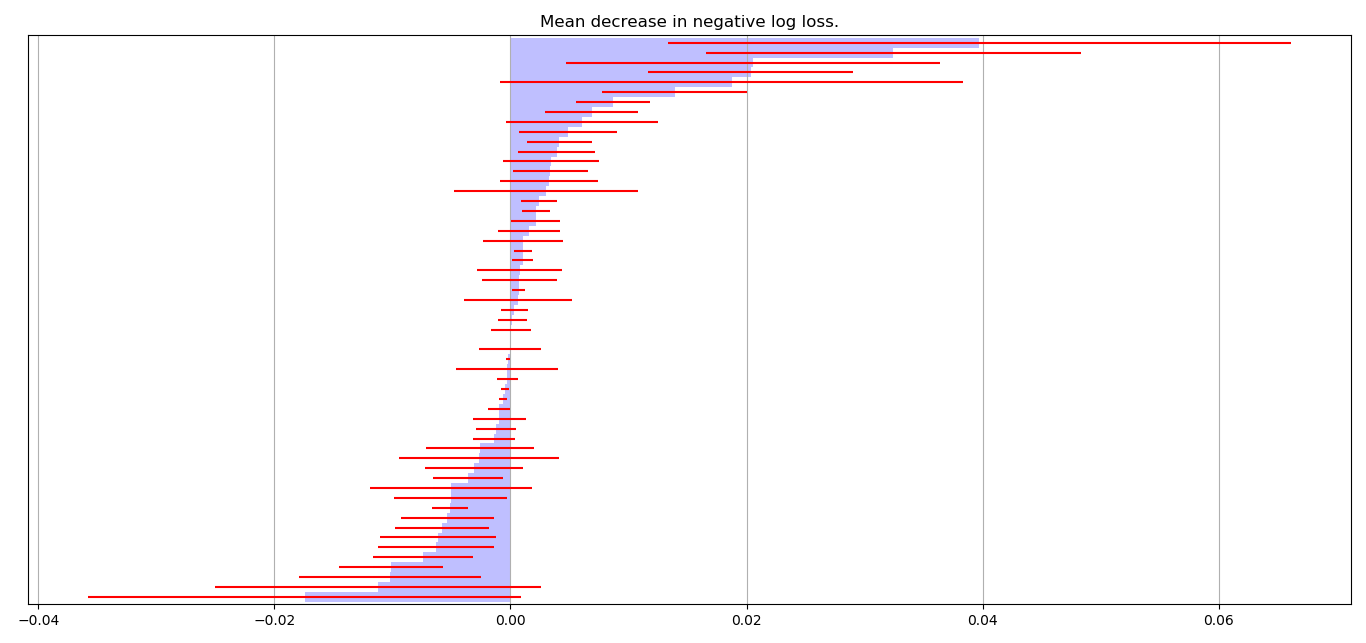
\includegraphics[width=1.35\textwidth, height=\textheight, keepaspectratio, angle=90]{results/images/feat_importance.png}
    \caption{Displays the mean feature importance loss in the bars. Each bar shows one feature. From the top to the bottom, there is one bar per feature in table \ref{table:feature_importance_results} and the rest are unimportant features. The standard deviation across cross validation folds is shown as a red line centered in the mean of each feature.}
    \label{fig:feat_importance}
\end{figure}

A new model was retrained using only these features. That model yields the results
in paragraph \emph{Performance metrics}. Also, as commented in
\ref{sec:methods_pipeline_feature_importance} it is important to explain how
these features are able to produce excess returns. It can be seen that price
related features are the ones that generate the higher mean of performance loss
and it means that a lot of market information is in prices already. Secondly, we
interpret that transacted volumes, both in currency and in bitcoins provide a lot
of information about market tendencies. As outlined in section \ref{sec:methods_features_sadf}
SADF related features determine when regime changes in price series occur and even
though that information is in prices, SADF offers a series that provides direct
information about changes towards explosive behavior. It is not surprising that
the day count until halving provides information and that is also connected with
the two volatility series. We have seen that close to halvings when
issuance changes and produces a considerable change in the network and that definitely
affects market volatility. Market capitalization offers an overall high level
market metric which provides an aggregated indicator of the market and similarly
does the transfer volume which accounts for the amount of currency that is flowing.
Making partitions over these features by means of a tree based model as bagging
ensembles are allows to generate complex relationship between them and identify
patterns. 

\paragraph{Performance metrics} Table \ref{table:perf_secondary_model}
shows the F1-score and negative log loss of the retrained secondary model.

\begin{table}[H]
  \centering
  \begin{tabular}{|c | c |} 
    \hline
    \multicolumn{2}{|c|}{Secondary model performance} \\
    \hline
    Metric & Value \\
    \hline
    F1-score                & 0.1574 \\
    \hline
    Negative log loss       & 0.6031 \\
    \hline
  \end{tabular}
  \caption{Secondary model classification metrics.}
  \label{table:perf_secondary_model}
\end{table}

F1-score evaluates model's accuracy when classifying samples. Negative log-loss
evaluates model's accuracy of the the estimated probabilities. The secondary
model will not be used as a classifier. Instead, predicted probabilities will
determine the bet size.
\subsection{Strategy results}
\label{sec:results_strategy}

Table \ref{table:financial_metrics} shows the results of the benchmark and the
strategy under test. We can see that the estimate on the Sharpe Ratio is bigger
for benchmark than the strategy under test. Later, evaluation of the
Probabilistic Sharpe Ratio will be used to analyze the confidence on the Sharpe
Ratio estimation for different reference values. Sortino ratio is bigger for the
strategy under test which is aligned with the win loss ratio observation. There
are no considerable differences in other indexes with the exception of the
volatility which has a rough difference of two magnitude orders.

Two indices were not computed for the benchmark strategy: correlation to
underlying (because it would be equal to 1) and the return on execution cost.
The latter will just add noise because only two trades will be executed: one at
the start of the time series and one at the end. Finally, because of the low
observed correlation value we can state that both strategies are doing quite
different things.

\begin{table}[H]
  \centering
  \begin{tabular}{| c | c | c |} 
    \hline
    \multicolumn{3}{|c|}{Financial metrics} \\
    \hline
    Metric & Buy and hold & Strategy under test \\
    \hline
    Sharpe ratio & 2.2156 & 1.2289 \\
    \hline
    Sortino ratio & 2.9138 & 5.7169 \\
    \hline
    Win loss ratio & 1.1171 & 8.0973 \\
    \hline
    Win rate & 0.5637 & 0.5833 \\
    \hline
    Average return & 0.0073 & 0.0065 \\
    \hline 
    Volatility & 1.2062 & 0.0352 \\
    \hline
    Correlation to underlying &  - & 0.0454 \\
    \hline
    Return on execution costs & - & 21.2264 \\
    \hline
  \end{tabular}
  \caption{Financial metrics benchmark.}
  \label{table:financial_metrics}
\end{table}

\begin{figure}[H]
    \centering
    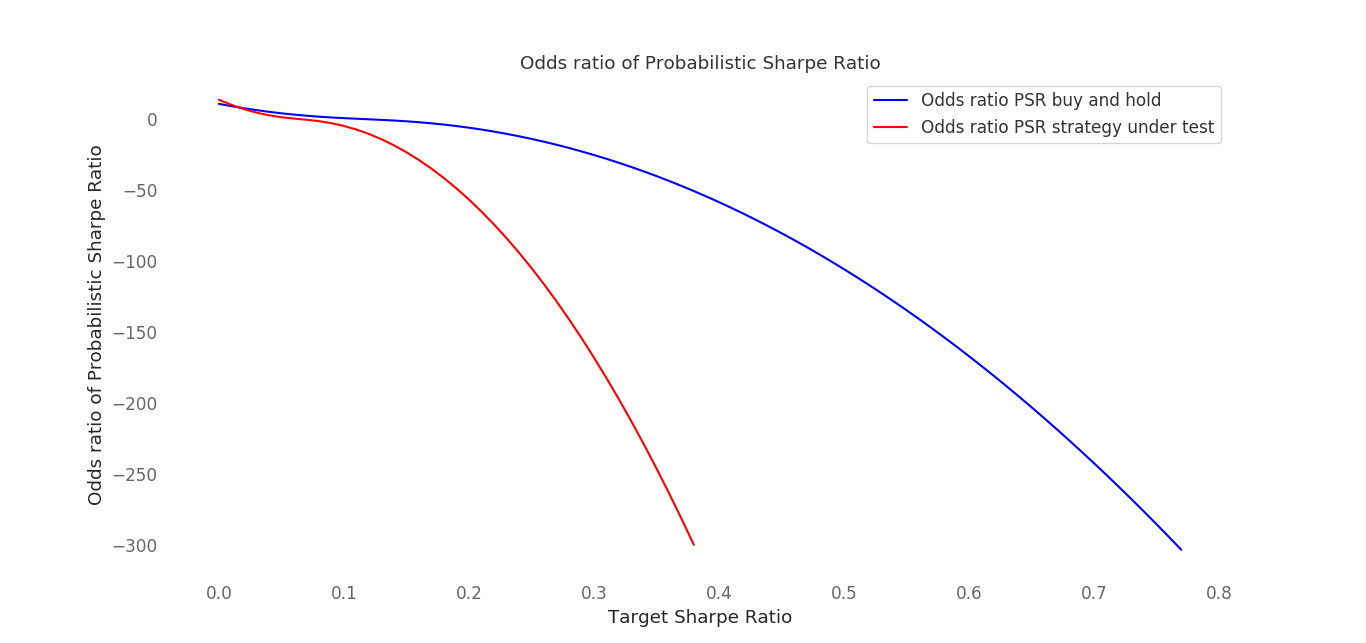
\includegraphics[width=\textwidth]{results/images/log_odds_ratio_psr.png}
    \caption{Odds ratio for the Probabilistic Sharpe Ratio of the buy and hold strategy and the strategy under test.}
    \label{fig:prob_sharpe_ratio}
\end{figure}

Because the Probabilistic Sharpe Ratio is compared against a sequence of target
Sharpe Ratios (0.01 increments between 0. and 1.), it is better shown in terms
log-odds ratio of the PSR values in figure \ref{fig:prob_sharpe_ratio}. It is observed
that for both strategies the odds quickly drop to quite low values below Sharpe
Ratios above 0.1. This is explained by analyzing the Probabilistic Sharpe Ratio
equation (\ref{eqn:prob_sharpe_ratio}). The denominator of the test statistic,
i.e. the standard error, is simply great because of the extremely large kurtosis
and skewness coefficients that both strategies exhibit. See table \ref{table:return_moments}
and remember that the normal distribution has a skewness of 0 and a kurtosis
of 3. Together with the table, figures
\ref{fig:b_h_return_distribution} and \ref{fig:st_return_distribution} display
histograms for the return distributions.

\begin{table}[H]
  \centering
  \begin{tabular}{| c | c | c |} 
    \hline
    \multicolumn{3}{|c|}{Moments of returns} \\
    \hline
    Metric & Buy and hold & Strategy under test \\
    \hline
    Mean of returns & 0.0073 & 0.0065 \\
    \hline
    Variance of returns & 0.0039 & 3.4018 . $10^{-6}$ \\
    \hline
    Skewness of returns & 0.2973 & 19.1115 \\
    \hline
    Kurtosis of returns & 11.9335 & 450.5218 \\
    \hline
  \end{tabular}
  \caption{Moments of the returns for both strategies}
  \label{table:return_moments}
\end{table}

\begin{figure}[H]
    \centering
    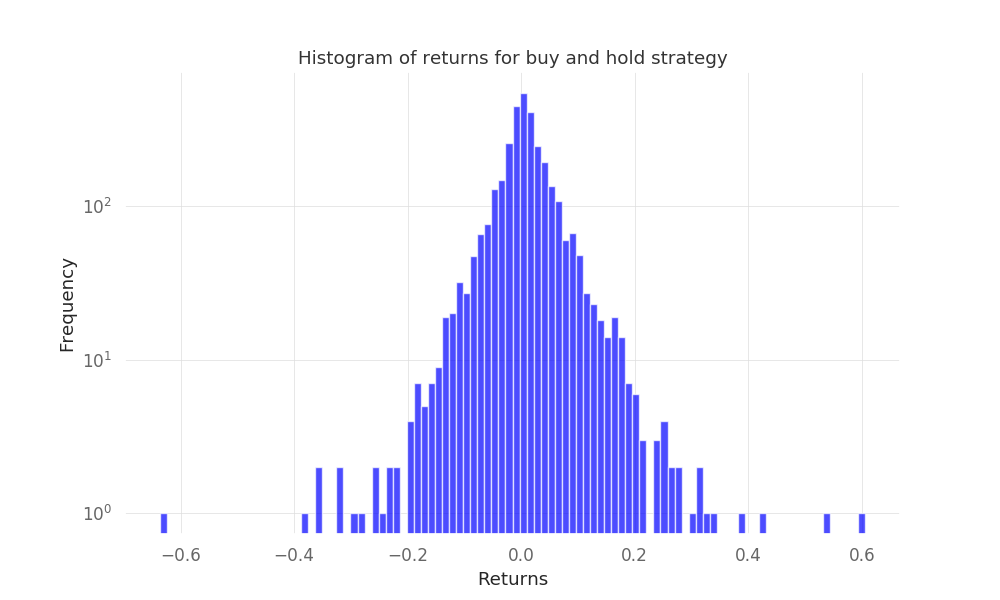
\includegraphics[width=1.1\textwidth]{results/images/hist_returns_btc.png}
    \caption{Buy and hold return distribution.}
    \label{fig:b_h_return_distribution}
\end{figure}

\begin{figure}[H]
    \centering
    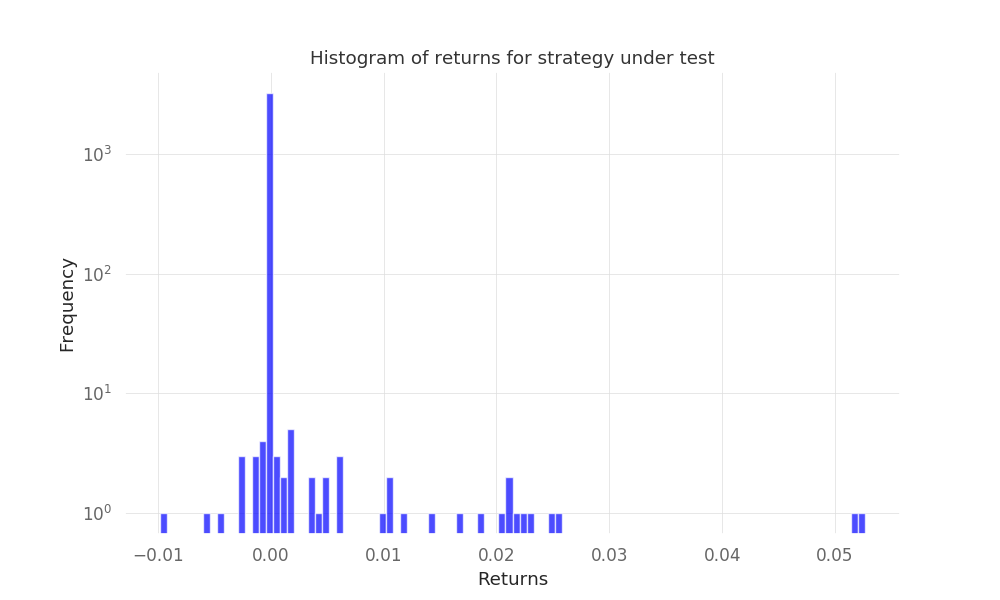
\includegraphics[width=1.1\textwidth]{results/images/hist_returns_st.png}
    \caption{Strategy under test return distribution.}
    \label{fig:st_return_distribution}
\end{figure}

\newpage
% @}

% @{ Conclusions
\section{Conclusion}
\label{sec:conclusion}

Along this research project a trading strategy over bitcoin with a machine
learning model to learn the bet size was developed and evaluated in modest but
comprehensive back testing benchmark. It was heavily based on the proposed
pipeline of Marcos Lopez de Prado and used some relatively novel variations to
a standard financial pipeline to test and evaluate a strategy. Careful feature
handling, rigorous training and validation techniques are described in each
section of this report.

The structure of this pipeline allows to change features, change a primary model,
change a secondary model or even the back testing strategy but preserve the other
building blocks because the interfaces are the same. The primary model should 
generate labels and metalabels to train a secondary model. The secondary model
will provide a probability to perform the bet sizing. Feature engineering will
be necessary to discard irrelevant features and explain the economic mechanism
why the strategy produces excess returns. The back testing could be more
comprehensive and incorporate new metrics but each stage preserves its interface.

As commented in \ref{sec:model_results} features from all the groups (price, volume, volatility, bitcoin network data, SADF indexes, and social indexes) remained in
the purged model except social indexes. Interest and animosity were removed
according to the heuristic rule to prune features that did not make a significant
impact on the performance loss. This result is important because it refuses one
of the preliminary intuitions for the secondary model. It was initially based on the belief
that knowing the social interest would affect the performance of the bet sizing
process. However, we probably assume that social indexes do not provide significant
new data that models can use because it is already incorporated into, e.g. prices.
On the contrary, a handful of SADF derived indexes remained and proved
to have higher mean loss of performance. Similarly, bitcoin ecosystem features and
traditional price and volume features remained in the final model.

Metrics for the secondary model performance are relatively bad ones compared to
other disciplines or domains. Also, as a classifier, it is by no means a good one.
However, the selection and training criteria that we used was to maximize the
negative log-loss of the model because the predicted probability is what
actually matters at the moment of implementing the strategy. It is worth noting
that even though a primary model with high accuracy can lead important losses if
the bet size is not properly computed when the primary model fails.

An increase in the negative log-loss is desired though and might be accomplished with further
analysis to the features. Lopez de Prado describes other techniques in chapter
8 of \cite{lopez_de_prado} to fight back the substitution effect that would lead
to the removal of important features. Also, with special care to overfitting, 
more complex machine learning models could be tested but that requires a back
testing scheme that stresses much more the strategy.

Section \ref{sec:results} provides a comprehensive set of metrics for each model
and the strategy as a whole. Some indicators lean towards
the strategy under test as it offers less volatility, higher win loss ratio
and Sortino ratio. However, the estimated Sharpe Ratio is smaller. When analyzing
the Probabilistic Sharpe ratio both strategies perform really bad and fall
rapidly when comparing them with different target ratios. Consequently, we 
cannot assure that they are considerably different based on the back testing evaluation.
It is also important to note that the Probabilistic Sharpe Ratio incorporates
a non-normality correction but the huge kurtosis and skewness coefficients make
the PSR probability to quickly drop.

\newpage
% @}

% @{ Future work
\section{Future work}
\label{sec:future_work}

In this section, we list some possible variations that could be applied to the
pipeline in the search for more performance.

\paragraph{Primary model} The primary model is using one of the many implementations
of momentum. Other alternatives can be tried using a relatively similar 
scheme and might lead to better results without affecting anything in the pipeline.
Furthermore, other non-momentum based primary models could be tried as well, e.g. mean reversion.
Anyway, any change to the primary model will imply retraining the secondary model
with the new labels.

The primary model can also be applied to more than one specific asset, like other
cryptocurrencies. That would provide more resilience to the secondary model because
it will be trained with labels and metalables generated from different asset sources
and reduce the risk of overfitting.

\paragraph{Secondary model} As mentioned in \ref{sec:conclusion}, other models
could be evaluated. Not only tree based models, but also neural networks or
SVMs. Probably, further feature engineering would be required for the latter two
and that would not necessarily be useful for the tree based models. Special
attentions should be paid to overfitting though. A more comprehensive back
testing strategy would be required aiming to evaluate the strategy under
more scenarios and realize if testing data produced in excess model adjustment.

\paragraph{Feature importance} Also, as commented in \ref{sec:conclusion}, 
it is recommended to try feature orthogonalization to mitigate the effect of
feature substitution (the analog of multi-collinearity in linear models) in the 
trees. Implementation of that technique was out of the scope of this research
project.

About interpretability, as Lopez de Prado points out in \cite{machine_learning_for_asset_managers}, only a theory can pin down
a cause-effect mechanism that allows you to generate excess returns. However,
most interpretability techniques are not suited for identifying causal
relationships unless additional assumptions are imposed (see \cite{causal_interpretations_of_bb_models}).  

At this time, interpretability techniques in machine learning have become a widely used tool for practitioners. However, their outputs must be taken only as approximations of what models are doing, even if those interpretability exercises are sufficient to comply with current regulatory constraints. In this regard, how to do proper inference on the estimates of feature importance remains a current research area.  In this regard, techniques for proper inference on the estimates of feature importance remain a current research area.

In another context, this point was also mentioned by Swadroe \cite{your_complete_guide_to_factor_investing} when he warns us to be skeptical about the persistence of excess returns from technical trading rules. These rules rely solely on historical prices and lack risk-based explanations that cannot be arbitraged away.


\paragraph{Back testing} The implemented back testing strategy is not the only
one that could be used and probably it is not the most appropriate, although the
most common. Splitting the feature space into multiple folds and mixing them
to create different time lines that the model could face is one the many alternatives
that would help to create different scenarios to evaluate the model.

There are several ways to obtain rich scenarios under which to stress a given strategy. For example,  with access to large data sets, Wiese, Knobloch, Korn, and Kretschmer in \cite{quant_gans} implement generative models for these purposes.

It is possible to analyze if more sophisticated back testing techniques are warranted by calculating a metric called  Probability of Backtest Overfitting (PBO, \cite{lopez_de_prado}).  This metric measures the change in performance rankings for our strategies.  In particular, one can use them when assessing different trading rules.   Intuitively, an optimal trading rule overfits when it is expected to underperform the median of a set of alternative trading rules out of the sample.

\paragraph{Metrics} In Andrew Lo \cite{the_statistics_of_sharpe_ratio} it is
shown how the simplified scale of from monthly Sharpe Ratios to annual Sharpe
Ratios cannot be simply expanded by $\sqrt{12}$ and it depends on its
distribution. Application of the proposed equations to the benchmark would correct
the informed Sharpe Ratio even more. 


\newpage
% @}

% @{ Future work
\section{Appendix}
\label{sec:appendix}

\subsection{Code}
\label{sec:appendix_code}

The code in this project is available on \href{https://github.com/agalbachicar/swing_for_the_fences}{https://github.com/agalbachicar/swing\_for\_the\_fences} and licensed under BSD 3-Clause "New" or "Revised" License. You can 
find in this \href{https://tldrlegal.com/license/bsd-3-clause-license-(revised)}{link}
what you can and cannot do with it. In the \emph{src} folder you will find:

\begin{itemize}
  \item bet\_sizing.py: contains functions to perform the bet sizing procedures explained in section \ref{sec:methods_pipeline_bet_sizing}
  \item btc\_strategy.py: contains many functions and classes that act as wrappers and implement the pipeline.
  \item cv.py: contains cross validation functions and classes that implement the purged $K$-fold cross validation with embargo. See section \ref{sec:methods_pipeline_training} for a reference about the techniques.
  \item events.py: contains functions that allow to obtain the labels by means of a momentum strategy. See section \ref{sec:methods_pipeline_primary_model}.
  \item feature\_importance.py: contains functions to evaluate the mean feature importance loss. See section \ref{sec:methods_pipeline_feature_importance}.
  \item features.py: contains functions to compute financial features out of a price series. See section \ref{sec:methods_features_fundamental}.
  \item frac\_diff.py: contains functions that implement the fractional differentiation method. See section \ref{sec:methods_features}.
  \item labelling.py: contains functions to implement labels and metalabels for price series. See section \ref{sec:methods_pipeline_primary_model}.
  \item load\_data.py: contains functions to load and merge datasets.
  \item mpfin.py: contains functions from chapter 20 of \cite{lopez_de_prado} for parallel execution of certain algorithms.
  \item pipeline\_thesis.py: main Python script to run and evaluate different stages of the pipeline.
  \item sample\_weights.py: contains functions to implement sample weights. See section \ref{sec:methods_pipeline_secondary_model}.
  \item sharpe\_ratio\_stats.py: contains functions to compute Sharpe Ratio and Probabilistic Sharpe Ration. See section \ref{sec:methods_pipeline_backtesting}.
  \item strategy\_backtesting.py: implements the back testing strategy and obtains results. See \ref{sec:methods_pipeline_backtesting} and \ref{sec:results}.
  \item structural\_breaks.py: contains functions to compute SADF series. See section \ref{sec:methods_features_sadf}. 
\end{itemize}

\emph{src/notebooks} folder contains some Jupyter Python notebooks to generate the images in this research project.

\emph{datasets} folder contains all datasets used in this project. Also, \emph{pickle} files with models, metrics and hyperparameter values are stored there by default for convenience.

\emph{doc} folder contains the latex project to generate this document.

\newpage
% @}
\printbibliography[heading=bibintoc, title={Bibliography}]
\newpage

\end{document}
% A Quantamental approach to Bitcoin trading: Are we swinging for the Fences?